\documentclass[12pt]{report}
\usepackage{verbatim}
\usepackage{fullpage}
\usepackage{etoolbox}
\usepackage{lipsum}
\usepackage{graphicx}
\usepackage{hyperref}
\usepackage{titlesec}
\usepackage{pdftexcmds}
\usepackage{minted}


\graphicspath{ {res/} }
\setcounter{secnumdepth}{4}
\titleformat{\paragraph}
{\normalfont\normalsize\bfseries}{\theparagraph}{1em}{}
\titlespacing*{\paragraph}
{0pt}{3.25ex plus 1ex minus .2ex}{1.5ex plus .2ex}

\newcommand{\HRule}{\rule{\linewidth}{0.5mm}}
\renewcommand\emph{\textbf}
\renewcommand{\baselinestretch}{1.1}

\newcommand{\printSQLtest}[1]
{
    \inputminted[linenos, breaklines, breakbytoken, tabsize=4, fontsize=\footnotesize]{mysql}{#1}
}

\newcommand{\printPHPImpl}[1]
{
    \inputminted[linenos, breaklines, breakbytoken, tabsize=4, fontsize=\footnotesize]{php}{#1}
}

\newcommand{\printPHP}[1]
{
    \printPHP{../www/php/#1}
}

\newcommand{\printSQLTablepage}[2]
{    
    \subsection{#2}
    \subsubsection{Code}
    \printSQLtest{../sql/parts/#1}
    \subsubsection{Explanation}
}

\begin{document}
    \begin{titlepage}

        \center

        \textsc{\LARGE Universita' degli Studi di Messina}\\[0.1cm]
        \textsc{\Large Dipartimento di Matematica e Informatica}\\[0.5cm]
        \textsc{\Large Database course project}\\[0.5cm]

        \HRule \\[0.4cm]
        { \huge \bfseries veeForum}\\[0.1cm]

        {\large 29 May 2015}
        \HRule \\[1.5cm]

        \begin{minipage}{0.4\textwidth}
        \begin{flushleft} \large
        \emph{Author:}\\
        Vittorio \textsc{Romeo}
        \end{flushleft}
        \end{minipage}
        ~
        \begin{minipage}{0.4\textwidth}
        \begin{flushright} \large
        \emph{Professor:} \\
        Massimo \textsc{Villari}


        \end{flushright}
        \end{minipage}\\[4cm]

        \vfill

        \begin{minipage}{\linewidth}
            \centering
            \begin{minipage}{0.35\linewidth}
                \begin{figure}[H]
                    \center
                    
\includegraphics[width=2cm, height=2cm]{logovee}

                    http://vittorioromeo.info
                \end{figure}
            \end{minipage}
            \hspace{0.27\linewidth}
            \begin{minipage}{0.35\linewidth}
                \begin{figure}[H]
                    \center
                    
\includegraphics[width=2cm, height=2cm]{logounime}

                    http://unime.it
                \end{figure}
            \end{minipage}
        \end{minipage}\\[3cm]
    \end{titlepage}

    \pagenumbering{gobble}
    \newcommand{\atoc}[1]{\addtocontents{toc}{#1\par}}
    \renewcommand{\thesection}{\arabic{section}.}
    \tableofcontents
    \newpage
    \pagenumbering{arabic}

    \part{Project specifications}
        The following part of the document describes the project and its design/development process without exploring its implementation details.

        The part begins with a synthesis of the \emph{client request}. After a careful analysis of the request, a \emph{Software Requirements Specification} (SRS) was written.

        Writing a correct and informative SRS is of utmost importance to achieve an high-quality final product and ensuring the development process goes smoothly.

        The SRS will cover the following points in depth:

        \begin{itemize}
            \item \emph{Scope and purpose}.
            \item \emph{Feature and functions}.
            \item \emph{External interface requirements}.
            \item \emph{Functional requirements}.
            \item \emph{Example use cases}.
            \item \emph{Non-functional requirements}.
            \item \emph{Analysis models}.
        \end{itemize}

        \chapter{Client request}

            The client requests the design and implementation of a \emph{forum creation/management framework} and a \emph{modern responsive web forum browsing/management application}.

            The client intends using the requested forum framework \emph{to build communication platforms} for various projects, both for internal employee usage and interaction with the public.

            It is imperative for the system to allow administrators to easily well-organized create \emph{content-section hierarchies} and \emph{user-group hierarchies}.

            Administrators also need to be able to \emph{give groups specific permissions for every section}.

            Some sections will only be visible and editable to employee groups (e.g. internal discussion), some sections will be visible but not editable by the public (e.g. announcements), and others will need to be completely open to the public (e.g. technical support).

            Being able to \emph{keep track of user-created content} is also very important for the client.

            Initially, tracking the date and the author of the content will be enough, but the system has to be designed in such a way that inserting additional creation information (e.g. browser/operating system used to post) will be trivial.

            In the future, additional content types (e.g. videos, attachments) may be added to the system and their creation will have to be tracked as well.

            Users and moderators will also need to be able to track user content through a \emph{real-time notification system} directly from the web application interface.

            This data needs to be independent from the contents, in order to easily allow administrators and project managers to gather statistical data on forum usage.

            The web application has to be extremely simple but flexible as well. Administrators need be able to perform all functions described above through a responsive admin panel.

            Content consumers and creators should be able to view and create content from the same responsive interface.

            Moderators and administrators should be able to edit and delete posts through the same interface as well. User interface controls will be shown/hidden depending on the user’s permissions.

        \chapter{Software Requirements Specification}


            \section{Introduction}

                \subsection{Software engineering}

                    \emph{Software engineering} is the study and an application of engineering to the design, development, and maintenance of software.

                    The Bureau of Labor Statistics' definition is Research, design, develop, and test operating systems-level software, compilers, and network distribution software for medical, industrial, military, communications, aerospace, business, scientific, and general computing applications.

                    Typical formal definitions of software engineering are:

                    \begin{itemize}
                        \item The systematic application of scientific and technological knowledge, methods, and experience to the design, implementation, testing, and documentation of software.
                        \item The application of a systematic, disciplined, quantifiable approach to the development, operation, and maintenance of software.
                        \item An engineering discipline that is concerned with all aspects of software production.
                        \item The establishment and use of sound engineering principles in order to economically obtain software that is reliable and works efficiently on real machines.
                    \end{itemize}   

                    \subsubsection{Background}

                        The term \emph{software engineering} goes back to the '60s, when more complex programs started to be developed by teams composed by experts.

                        There was a radical transformation of software: from \emph{artisan product} to \emph{industrial product}.

                        A software engineer needs to be a good programmer, an algorithm and data structures expert with good knowledge of one or more programming languages.

                        He needs to know various design processes, must have the ability to convert generic requirements in well-detailed and accurate specifications, and needs to be able to communicate with the end-user in a language comprehensible to him comprehensible.

                        Software engineering, is, however, a discipline that's still evolving. There still are no definitive standards for the software development process.

                        Compared to traditional engineering, which is based upon mathematics and solid methods and where well-defined standards need to be followed, software engineering is greatly dependent on personal experience rather than mathematical tools.

                        Here's a brief history of software engineering:

                        \begin{itemize}
                            \item \emph{1950s}: Computers start to be used extensively in business applications.
                            \item \emph{1960s}: The first software product is marketed. 

                            IBM announces its unbundling in June 1969.
                            \item \emph{1970s}: Software products are now regularly bought by normal users. 

                            The software development industry grows rapidly despite the lack of financing.

                            The first software houses begin to emerge.
                        \end{itemize}

                    \subsubsection{Differences with programming}

                        \begin{itemize}
                            \item A programmer writes a complete program.
                            \item A software engineer writes a software component that will be combined with components written by other software engineers to build a system.
                        \end{itemize}

                        \begin{itemize}
                            \item Programming is primarily a personal activity.
                            \item Software engineering is essentially a team activity.
                        \end{itemize}

                        \begin{itemize}
                            \item Programming is just one aspect of software development.
                            \item Large software systems must be developed similar to other engineering practices.
                        \end{itemize}

                \subsection{SRS}

                    This \emph{Software Requirements Specification} (SRS) chapter contains all the information needed by software engineers and project managers to design and implement the requested forum creation/management framework.

                    The SRS was written following the \emph{Institute of Electrical and Electronics Engineers} (IEEE) guidelines on SRS creation.

                \subsection{Purpose}
                    The SRS chapter is contained in the \emph{non-technical} part of the thesis.

                    Its purpose is providing a \emph{comprehensive description} of the objective and environment for the software under development.

                    The SRS fully describes \emph{what the software will do} and \emph{how it will be expected to perform}.

                \subsection{Scope}

                    \subsubsection{Identity}
                        The software that will be designed and produced will be called \emph{veeForum}.

                    \subsubsection{Feature extents}

                        The complete product will:

                        \begin{itemize}
                            \item Provide a framework for the \emph{creation and the management of a forum system}.
                            \item Allow its users to \emph{deploy and administrate} multi-purpose forums.
                            \item Give access to a \emph{modern responsive web application} to setup, browse and manage the forum.
                        \end{itemize}

                        veeForum, however, will not:

                        \begin{itemize}
                            \item Provide infrastructure or implementation for a complete blog/website. The scope of the software is forum building.
                            \item Implement instant private messaging - user-to-user chat is beyond the scope of the project.
                        \end{itemize}

                    \subsubsection{Benefits and objectives}

                        Deploying veeForum will give its users a number of important benefits and will fulfill specific objectives.

                        \begin{itemize}
                            \item Companies and individuals making use of veeForum will have access to an \emph{easy-to-install} and \emph{easy-to-use} forum creation and management platform.
                            \item Users and moderators of the deployed forums will be able to \emph{easily create, track and manage} content and other forum users.
                            \item Forum administrators will be given \emph{total control} of the forum structure, users and permissions through an \emph{easy-to-use} responsive administration panel.
                        \end{itemize}

            \section{General description}
                \subsection{Product perspective and functions}
                    The product shares many basic aspects and features with existing forum frameworks such as \emph{phpBB} or \emph{vBulletin}: flat/threaded discussion support, nested sections, user attachments, etc.

                    veeForum improves on existing forum frameworks in the following ways:

                    \begin{itemize}
                        \item Provides a responsive web interface without postbacks.
                        \item Allows users and moderators to subscribe and unsubscribe not only to posts, but to users and sections as well.
                        \item Has a powerful \emph{real-time} Facebook-like notification system that notifies users when tracked content has been added or edited.
                        \item Gives administrator the possibility to \emph{design and manage complex permission hierarchies} for user groups and single users.
                    \end{itemize}

                \subsection{User characteristics}
                    veeForum needs to target both users that \emph{only consume the content offered by deployed forums}, users that \emph{actively create and manage content in deployed forums}, and users that \emph{build and deploy forum instances}.

                    User-friendliness is essential for every target, but all the required functionality is effectively exposed to different user groups.

                    It is therefore required to have clear interfaces thar do not negatively affect the user experience by being either too complex or too simple (all features need to be exposed).

            \section{Specific requirements}

                \subsection{External interface requirements}

                    \emph{External interface requirements} identify and document the interfaces to other systems and external entities within the project scope.

                    \subsubsection{User interfaces}
                        The product will provide both a desktop and a mobile user web interface.

                        \begin{itemize}
                            \item \emph{Web interface}: it is required to provide a modern responsive web interface, compatible and tested with the most popular browsers (Internet Explorer 10+, Google Chrome, Mozilla Firefox). The web interface will give forum access to users and moderators, and administrator access to forum management staff.
                            \item \emph{Mobile interface}: is is required to provide a modern mobile application for the major platforms (Android, iOS, Windows Phone). The mobile application will allow browsing and content management of forums created with the product.
                        \end{itemize}

                    \subsubsection{Software interfaces}
                        The \emph{open-source policy} of veeForum will allow framework users to expand or improve existing functionality and to interact with other existing technologies.

                        Accessing and modifying forum data (assuming permission requirements are satisfied by the user) will be possible through \emph{RESTful} requests, returning and accepting \emph{JSON} (Javascript Object Notation).

                \subsection{Functional requirements}
                    In software engineering, a \emph{functional requirement} defines a function of a system and its components.

                    Functional requirements may be \emph{calculations}, \emph{technical details}, \emph{data manipulation and processing} and other specific functionality that define what a system is supposed to accomplish.

                    Behavioral requirements describing all the cases where the system uses the functional requirements are captured in \emph{use cases}.

                    \subsubsection{User/group management}
                        \begin{itemize}
                            \item \emph{Users}: users will be managed by the system. Users can register (or be manually added by an administrator). Registration can be configured to require a confirmation email or not.
                            \item \emph{Groups}: every user will be part of at least one group at all times. Groups are part of an hierarchy: they can inherit from each other. Groups can have permissions specific to sections and system-wide permissions.
                        \end{itemize}

                        \begin{figure}[!htb]
                        \caption{User/group hierarchy example.}
                        \centering
                        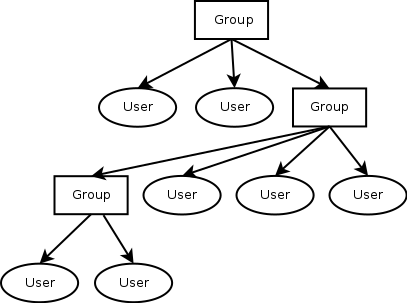
\includegraphics[width=0.5\textwidth]{ed/hier_user}
                        \end{figure}

                     \subsubsection{Content hierarchy}
                        \begin{itemize}
                            \item \emph{Posts}: posts will be the base of the content hierarchy. They will contain HTML-enabled text and any number of attachments.
                            Posts can be edited and deleted by the original owner.
                            \item \emph{Threads}: threads are groups of posts. Users with the correct permissions can create a thread in a specific section and have other users add posts or subscribe to it.
                            Threads can be edited and deleted by the original owner.
                            \item \emph{Sections}: sections are content containers intended to group threads related to the same subject. Forum administrators and moderators can create sections and give users permissions to view or edit them.
                            \item \emph{Attachments}: users with the correct permissions can upload files and attach any number of them to one of their posts.
                        \end{itemize}

                        \begin{figure}[!htb]
                        \caption{Content hierarchy example.}
                        \centering
                        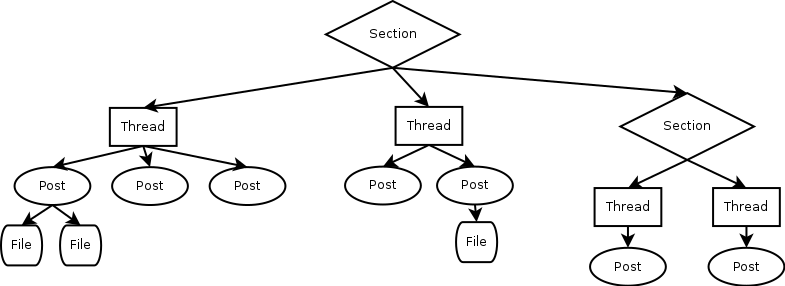
\includegraphics[width=1\textwidth]{ed/hier_sec}
                        \end{figure}

                      \subsubsection{Content tracking system}
                        \begin{itemize}
                            \item \emph{Creation data}: user-created content (posts, threads,attachments, etc) will have some data specific to its creation can be extended by forum administrators. Basic predefined data will consist of creation date and time. It will be possible to run statistical queries on content creation data.
                            \item \emph{Subscriptions}: users and moderators will be able to subscribe to specific sections, threads or user to track their contents. They will receive real-time notifications upon addition/editing of tracked content.
                        \end{itemize}

                        \begin{figure}[!htb]
                        \caption{Subscription/notification architecture example.}
                        \centering
                        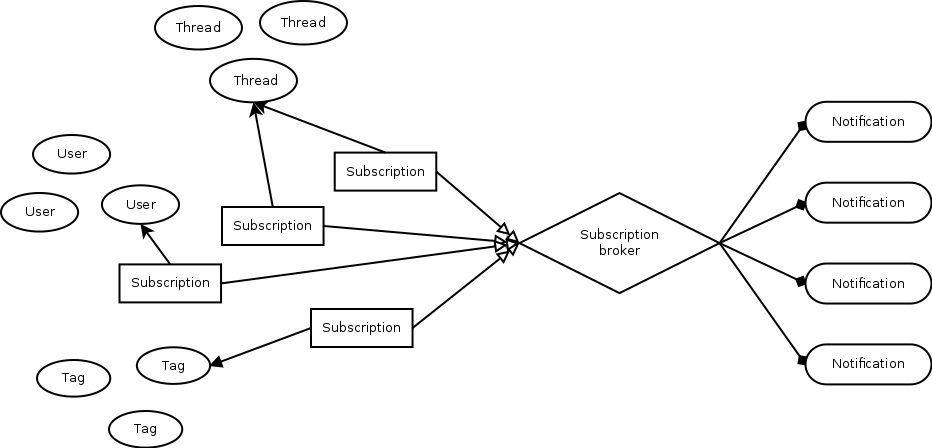
\includegraphics[width=1\textwidth]{ed/hier_sub}
                        \end{figure}

                \newpage

                \subsection{Example use cases}
                    In software and systems engineering, a \emph{use case} is a list of steps, typically defining interactions between one or more actors and a system, to achieve a goal.

                    \subsubsection{Mobile game forum}
                        A company developed a popular mobile game, with a wide audience.
                        The company uses the \emph{veeForum framework} to give users a place to discuss game strategy, give feedback on the quality of their product and receive technical support.

                        \paragraph{Actors}
                            \begin{itemize}
                                \item Game developers.
                                \item Game players.
                                \item Forum management team.
                                \item Technical support team.
                                \item Feedback (PR) team.
                            \end{itemize}

                        \paragraph{Pre-conditions}
                            \begin{itemize}
                                \item Release of a popular product with a wide audience.
                                \item Game users need to register on the forum.
                            \end{itemize}

                        \paragraph{Flow of events}
                            \begin{itemize}
                                \item Installation and configuration of a veeForum-enabled forum system by the forum management team.
                                \item Creation of the sections and permission hierarchies by the forum management team and the developers.
                                \item Registration and content creation by the game developers and game players.
                            \end{itemize}

                        \paragraph{Post-conditions}
                            \begin{itemize}
                                \item Game players will be able to share their strategies and thoughts on the product.
                                \item The technical support team will find all technical issues grouped in a convenient way and will be able to track individual issues. Technical support members will be able to communicate with each other in a private section.
                                \item The feedback team will be able to track user suggestions and forward potential product improvements to the developer team.
                            \end{itemize}

                        \begin{figure}[!htb]
                        \caption{Basic forum usage use case diagram.}
                        \centering
                        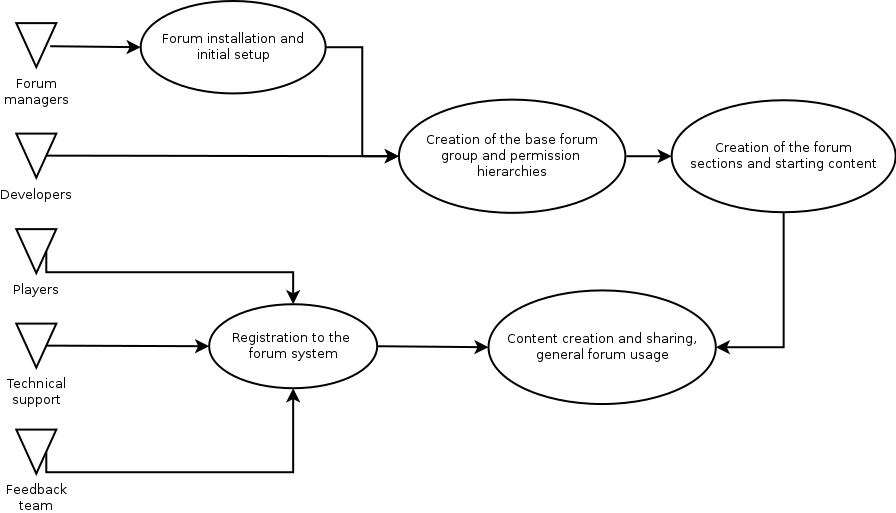
\includegraphics[width=1\textwidth]{uc/uc1}
                        \end{figure}

                        \begin{figure}[!htb]
                        \caption{Technical support and feedback use case diagram.}
                        \centering
                        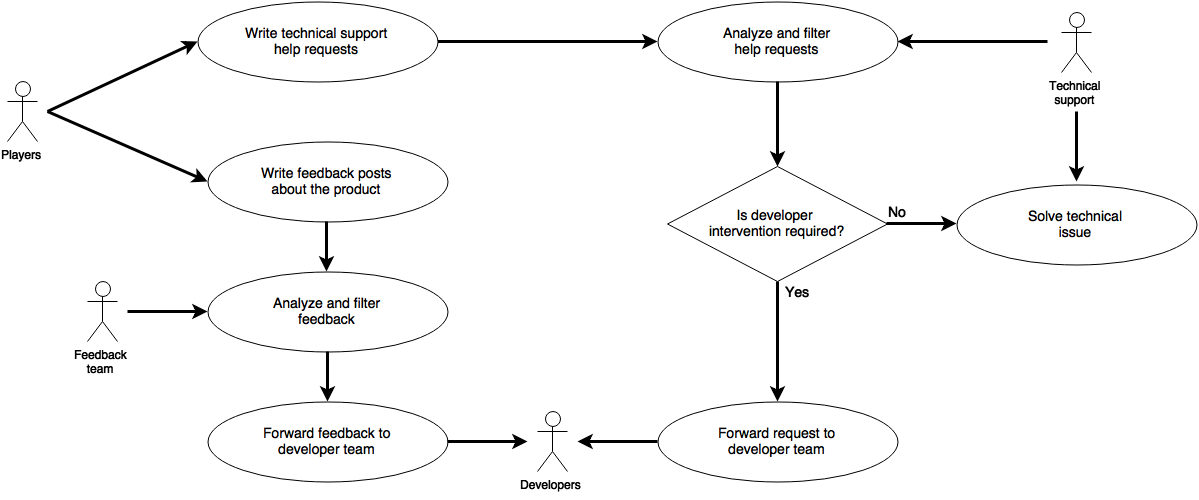
\includegraphics[width=1\textwidth]{uc/uc2}
                        \end{figure}

                    \newpage
                    \subsubsection{Local city GNU/Linux usergroup forum}
                        Some GNU/Linux users from the same city decide to start a local usergroup to discuss the GNU/Linux ecosystem and make new friends. In spirit with the open-source nature of the system, collaboration is extremely important. They require to easily assign specific permissions to users and groups to allow the forum to grow and be well-organized.

                        \paragraph{Actors}
                            \begin{itemize}
                                \item Usergroup creators.
                                \item Usergroup members.
                                \item External visitors.
                            \end{itemize}

                        \paragraph{Pre-conditions}
                            \begin{itemize}
                                \item Interest in a local GNU/Linux usergroup.
                                \item Availability of people willing to collaborate.
                            \end{itemize}

                        \paragraph{Flow of events}
                            \begin{itemize}
                                \item Installation and configuration of a veeForum-enabled forum system by the usergroup creators.
                                \item Creation of the initial sections and permission hierarchies by the usergroup creators.
                                \item Registration of usergroup members and external visitors.
                                \item The usergroup creators give other usergroup members permissions to create and manage sections and users, starting a chain of collaborative forum content development.
                                \item Usergroup members and external visitors contribute and make use of the content.
                            \end{itemize}

                        \paragraph{Post-conditions}
                            \begin{itemize}
                                \item Local city usergroup members will be able to get to know and speak to each other.
                                \item Usergroups members willing to contribute will be able to easily manage sections and write posts/articles.
                                \item External visitors will be able to make use of the public content.
                            \end{itemize}

                        \begin{figure}[!htb]
                        \caption{Usergroup forum use case diagram.}
                        \centering
                        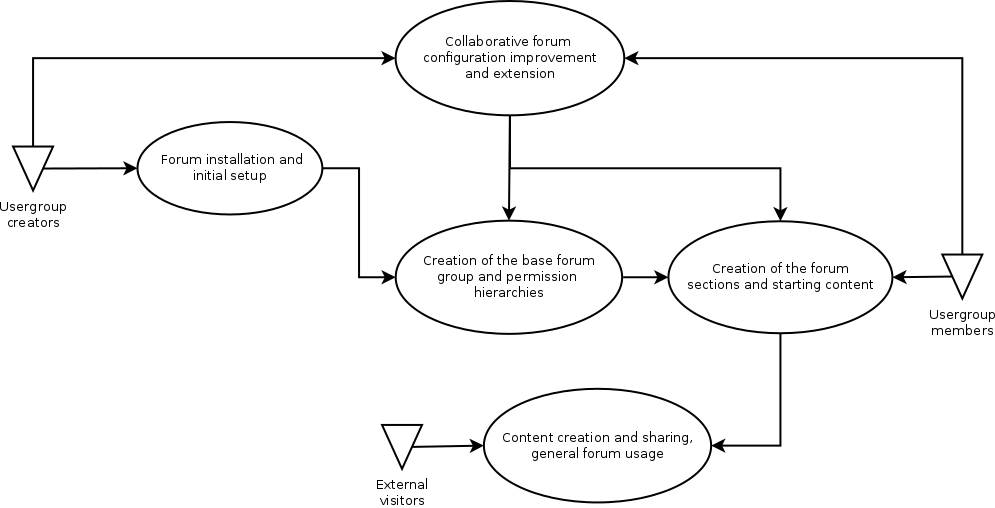
\includegraphics[width=1\textwidth]{uc/uc3}
                        \end{figure}

                \subsection{Non-functional requirements}
                    Functional requirements are supported by \emph{non-functional requirements} (also known as quality requirements), which impose constraints on the design or implementation (such as performance requirements, security, or reliability).

                    \subsubsection{Performance}
                        The system will be designed from the ground-up with emphasis on performance. As the forum may have huge amounts of contents and concurrent usage after its deployment, optimizing is a must.

                        When possible, functions will be implemented \emph{directly in the database}, for maximum performance.

                        Web backend functions will also be carefully \emph{optimized both for memory and speed}.

                    \subsubsection{Reliability}
                        The system will have to be reliable and keep working in case of errors.

                        Database queries and functions will be executed in \emph{safe wrappers} that catch and handle errors carefully.

                    \subsubsection{Security}
                        veeForum needs to guarantee privacy and security for users and administrator of the system.

                        Well-tested and well-received \emph{security idioms} and \emph{encryption algorithms} will have to be used throughout the implementation of the whole system.

                    \subsubsection{Maintainability and portability}
                        Being an open-source project, \emph{maintainability}, \emph{extensibility} and \emph{portability} are key.

                        The code layer will be carefully designed and organized to allow easy maintenance, bugfixing and feature addition.

                        To ensure maximum portability, the product will be designed to work on the most popular \emph{GNU/Linux} distributions and will be thoroughly tested on different platforms.
            
            \section{Analysis models}
                \subsection{Activity Diagrams}
                    Activity diagrams are graphical representations of workflows of stepwise activities and actions with support for choice, iteration and concurrency. 
                    In the Unified Modeling Language, activity diagrams are intended to model both computational and organisational processes (i.e. workflows). 
                    Activity diagrams show the overall flow of control.

                    \newpage

                    The following diagram shows the steps that the \emph{forum management team} must take in order to setup and initialize a veeForum-enabled forum.

                    \begin{figure}[!htb]
                    \caption{Forum setup and initialization activity diagram.}
                    \centering
                    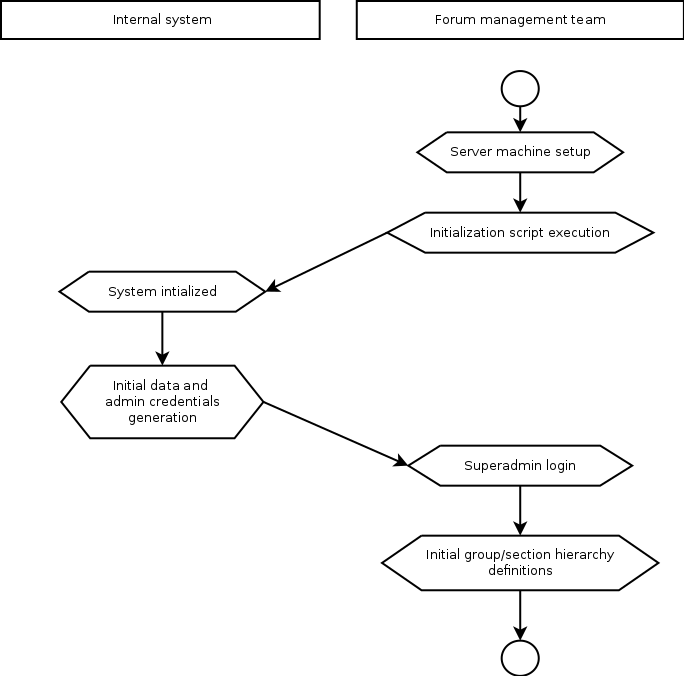
\includegraphics[width=1\textwidth]{uc/a1}
                    \end{figure}

                    \newpage

                    The following diagram shows the steps that the \emph{forum users} must take in order to add content to the forum system.

                    \begin{figure}[!htb]
                    \caption{Content creation activity diagram.}
                    \centering
                    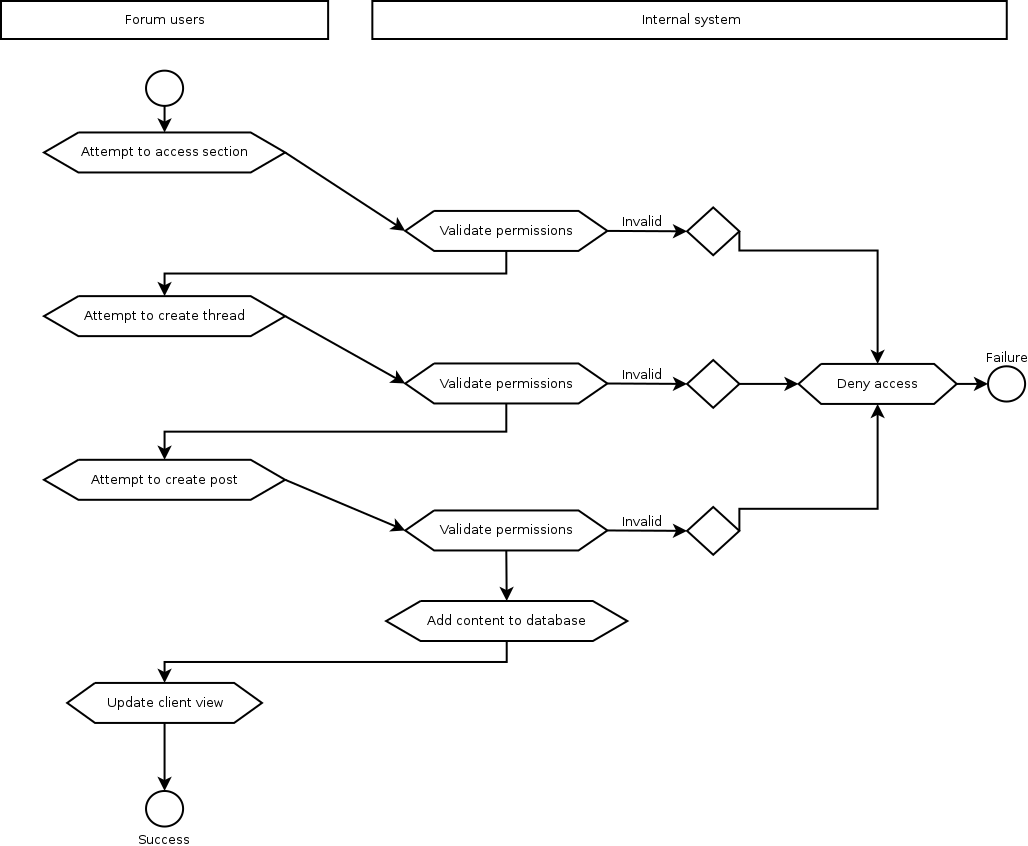
\includegraphics[width=1\textwidth]{uc/a2}
                    \end{figure}

                    \newpage

                \subsection{Sequence Diagrams}
                    
                    The following diagram shows the interaction between \emph{forum users}, the \emph{subscription broker} and the \emph{content management} systen in order to manage subscriptions and generate notifications.

                    \begin{figure}[!htb]
                    \caption{Subscription/notification system sequence diagram.}
                    \centering
                    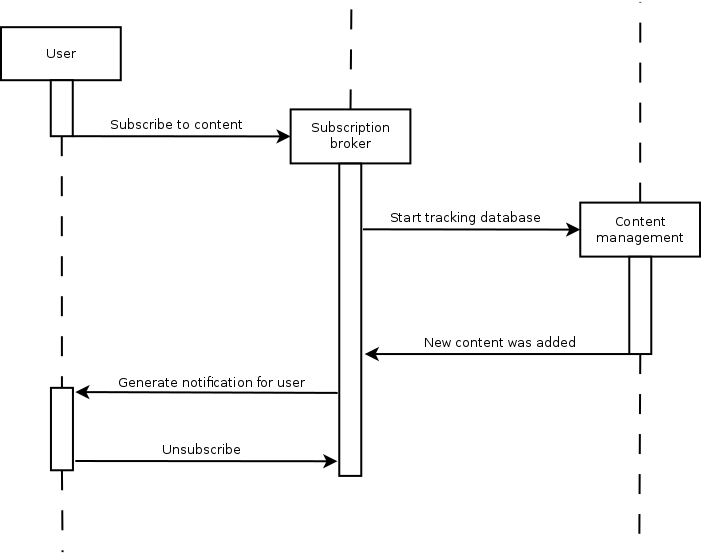
\includegraphics[width=1\textwidth]{uc/s1}
                    \end{figure}

                    \newpage

    \part{Technical analysis}
        The following part of the thesis will cover all implementation choices and details for veeForum in depth.

        Firstly, the \emph{development environment and tools} and \emph{chosen technologies} will be described and motivated.

        Afterwards, the technical details, including code examples and APIs, will be described for the two modules of the application: the \emph{database} and the \emph{web application}.

        Every \emph{table} of the database will be analyzed in detail, directly showing commented \emph{DDL} code. The database also contains important \emph{stored procedures} and \emph{triggers} that are core part of the system's logic and that need to be explained in depth - the related \emph{DML} code will be shown and commented.

        The web application itself is divided in multiple modules:
        \begin{itemize}
            \item A \emph{database interface backend module}, that interfaces with the database and wraps its tables and stored procedures.
            \item A \emph{HTML5 generation module}, that greatly simplifies the creation of dynamic forum web pages by wrapping HTML5 controls in \emph{object-oriented wrappers} that can be easily bound to callbacks and database events.
            \item A \emph{modern responsive AJAX frontend} that allows users and interact with the backend module from multiple device, limiting postbacks and page refreshes.
        \end{itemize}

        \chapter{Development process}

            \section{Environment and tools}
                All modules of veeForum have been developed on \emph{Arch Linux x64}, a lightweight GNU/Linux distribution.

                Arch is installed as a minimal base system, configured by the user upon which their own ideal environment is assembled by installing only what is required or desired for their unique purposes. GUI configuration utilities are not officially provided, and most system configuration is performed from the shell and a text editor. Based on a rolling-release model, Arch strives to stay bleeding edge, and typically offers the latest stable versions of most software.

                No particular integrated development environments (IDEs) were used during the development - a modern graphical text editor, \emph{Sublime Text 3}, was used instead.

            \section{Docker}
                Docker is an open-source project that \emph{automates the deployment of applications} inside software containers, by providing an additional layer of abstraction and automation of operating-system-level virtualization on Linux.

                Docker uses resource isolation features of the Linux kernel such as \emph{cgroups} and \emph{kernel namespaces} to allow independent containers to run within a single Linux instance.

                This technology has been used since the beginning of the development process to \emph{separate veeForum data and packages} from the host system and to dramatically increase \emph{portability} and \emph{ease of testing}.

                Docker is also used for the installation of the product on target systems - with a single command it is possible to \emph{retrieve all required dependencies}, correctly \emph{configure the system} and \emph{automatically install veeForum}.

            \section{Version control system}
                Version control systems (VCSs) allow the \emph{management of changes} to documents, computer programs, large web sites, and other collections of information.

                Nowadays, a version control system is \emph{essential} for the development of any project.
                Being able to track changes, develop features in separate \emph{branches}, have multiple programmers work on the same code base without conflicts and much more is extremely important for projects of any scope and size.

                The chosen VCS is \emph{Git}, a distributed revision control system with an emphasis on \emph{speed}, \emph{data integrity}, and support for \emph{distributed, non-linear workflows}.

                Git is widely appreciated in the private and open-source programming communities - it was initially designed and developed by \emph{Linus Torvalds} for Linux kernel development in 2005, and has since become the most widely adopted version control system for software development.

                The veeForum project is \emph{open-source} and \emph{appreciates feedback and contributions}. It is hosted on \emph{GitHub}, a web-based Git repository hosting service, which offers all of the distributed revision control and source code management (SCM) functionality of Git, while adding \emph{additional features} that make collaboration and public contributions easy and accessible.

            \section{LAMP stack}
                The server and web application run on a \emph{LAMP stack}, on a GNU/Linux machine.

                A LAMP stack is composed by the following technologies:

                \begin{itemize}
                    \item \emph{L}: GNU/Linux machine.
                    \item \emph{A}: Apache HTTP server.

                     The Apache HTTP server is the world's most widely used web server software.

                     Apache has been under open-source development for about 20 years - it supports all modern server-side technologies and programming languages, and also is \emph{extremely reliable} and \emph{secure}.

                    \item \emph{M}: Stands for MySQL server, but \emph{MariaDB}, a modern drop-in replacement for MySQL is used as the DBMS. 

                    MariaDB is fully compliant with the MySQL standard and language, but it is more performant and has additional features. It is the default DBMS in the Arch Linux distribution.

                    \item \emph{P}: PHP5, the server backend language. 

                    HTML5, PHP5 and JavaScript conformant to the 5.1 ECMAScript specification (along with the JQuery library) are used for the development of the web application. 

                    The \emph{AJAX} (Asynchronous JavaScript and XML) paradigm will be used to ensure that the application feels responsive and that user interaction is immediately reflected on the web application.

                \end{itemize}
               
            \section{Thesis}
                The current document was written using \LaTeX, an high-quality typesetting system; it includes features designed for the production of \emph{technical and scientific documentation}.

                \LaTeX{} was chosen for the current document because of the visually pleasant typography, its extensibility features and its abilities to include and highlight source code.

                \subsection{LatexPP}
                    A small \emph{C++14} \LaTeX{} preprocessor named \emph{LatexPP} was developed for the composition of this thesis.

                    LatexPP allows to use an intuitive syntax that avoids markup repetition for code highlighting and macros.

                    Preprocessing and compiling a \LaTeX{} document using LatexPP is simple and can be automated using a simple \emph{bash} script.

\begin{minted}[mathescape, linenos, numbersep=5pt, gobble=2, frame=lines, framesep=2mm, fontsize=\footnotesize]{bash}
    #!/bin/bash

    latexpp ./thesis.lpp > ./thesis.tex
    pdflatex -shell-escape ./thesis.tex && chromium ./thesis.pdf
\end{minted}

                    LatexPP is available as an open-source project on GitHub:

                    \url{https://github.com/SuperV1234/Experiments/Random}


        \chapter{Project structure}
            The project folder and file structure is organized as such:

            \begin{itemize}
                \item \emph{./doc/}

                    Folder containing the documentation of the project.
                    \begin{itemize}
                        \item \emph{./latex/}

                        LatexPP and \LaTeX{}  source and output files.
                    \end{itemize}

                \item \emph{./sql/}

                    Folder containing the SQL DDL scripts.
                    \begin{itemize}
                        \item \emph{./scripts/}

                        Contains all the parts that make up the complete SQL initialization script.

                        \item \emph{./mkScript.sh}

                        Builds the complete SQL initialization scripts from the files in ./scripts/.

                        \item \emph{./script.sql}

                        Complete SQL initialization scripts that sets up a database suitable veeForum.
                    \end{itemize}

                \item \emph{./exe/}

                    Folder containing executable scripts to setup the system.
                    \begin{itemize}
                        \item \emph{./docker/}

                        Docker-related scripts.
                        \begin{itemize}
                            \item \emph{./start.sh}

                            Starts a Docker instance containing veeForum.

                            \item \emph{./cleanup.sh}

                            Cleans any running veeForum Docker instance.

                            \item \emph{./shell.sh}

                            Starts a Docker instance containing veeForum, controlling an instance of bash inside it.

                            \item \emph{./httpdLog.sh}

                            Prints the Apache error log of the current running veeForum Docker instance.
                        \end{itemize}

                    \end{itemize}

                \item \emph{./www/}

                    Folder containing web application data.
                    \begin{itemize}

                        \item \emph{./css/}

                        CSS3 stylesheets.

                        \item \emph{./js/}

                        ECMAScript 5 script files.

                        \item \emph{./json/}

                        Non-relational data storage files, in JSON format.

                        \item \emph{./php/}

                        PHP backend code.
                        \begin{itemize}
                            \item \emph{./lib/}

                            Backend to database interface library and HTML5 generation library.

                            \item \emph{./core/}

                            PHP frontend files that generate the responsive HTML5 web application user interface.
                        \end{itemize}

                    \end{itemize}

            \end{itemize}

        \chapter{Database design}
            \section{Diagrams}

                \begin{figure}[!htb]
                \caption{Complete DB Entity-Relationship diagram.}
                \centering
                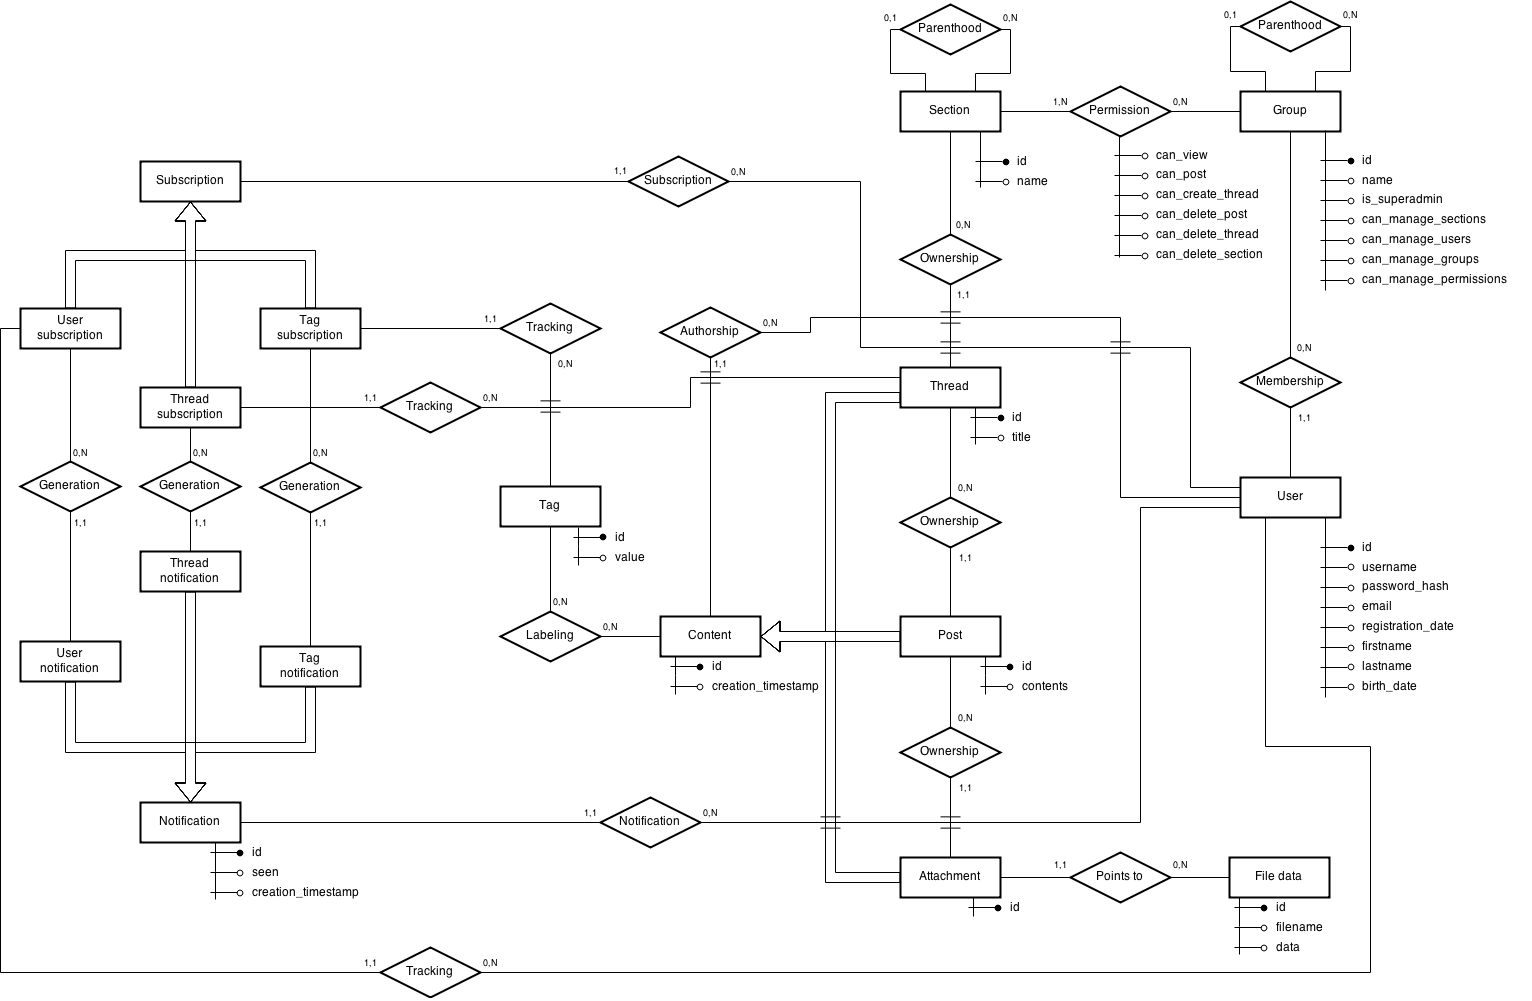
\includegraphics[width=1\textwidth]{erdiag}
                \end{figure}

                \begin{figure}[!htb]
                \caption{ER diagram zoom: content hierarchy}
                \centering
                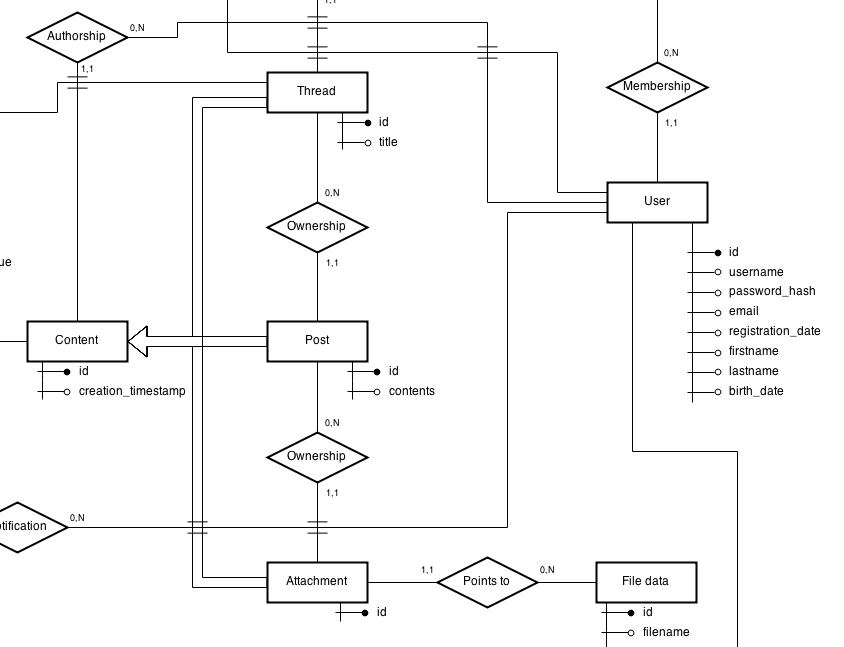
\includegraphics[width=1\textwidth]{erzm0}
                \end{figure}

                \begin{figure}[!htb]
                \caption{ER diagram zoom: section hierarchy}
                \centering
                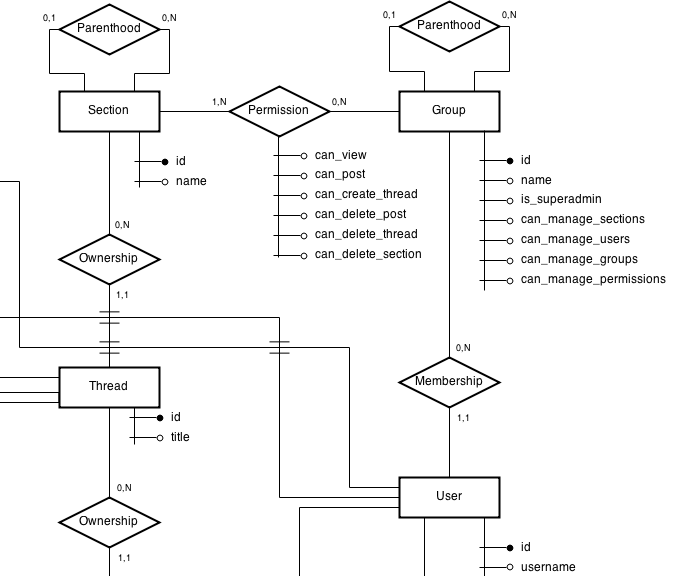
\includegraphics[width=1\textwidth]{erzm1}
                \end{figure}

                \begin{figure}[!htb]
                \caption{ER diagram zoom: content subscription/notification system}
                \centering
                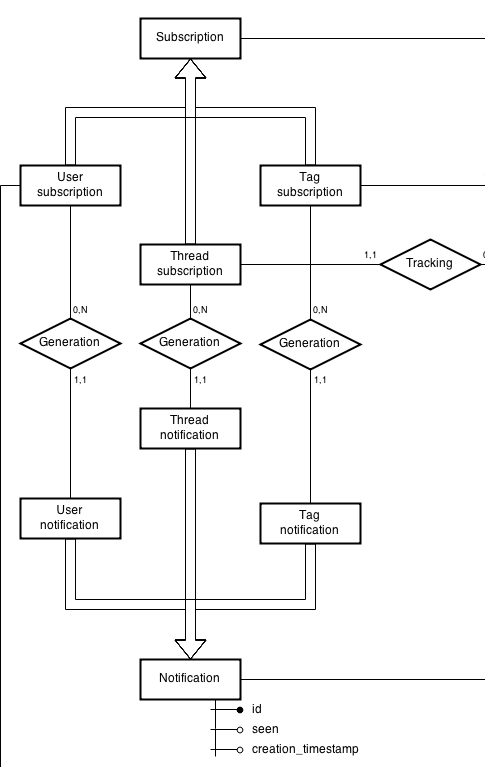
\includegraphics[width=0.7\textwidth]{erzm2}
                \end{figure}

                \begin{figure}[!htb]
                \caption{Complete DB logic diagram.}
                \centering
                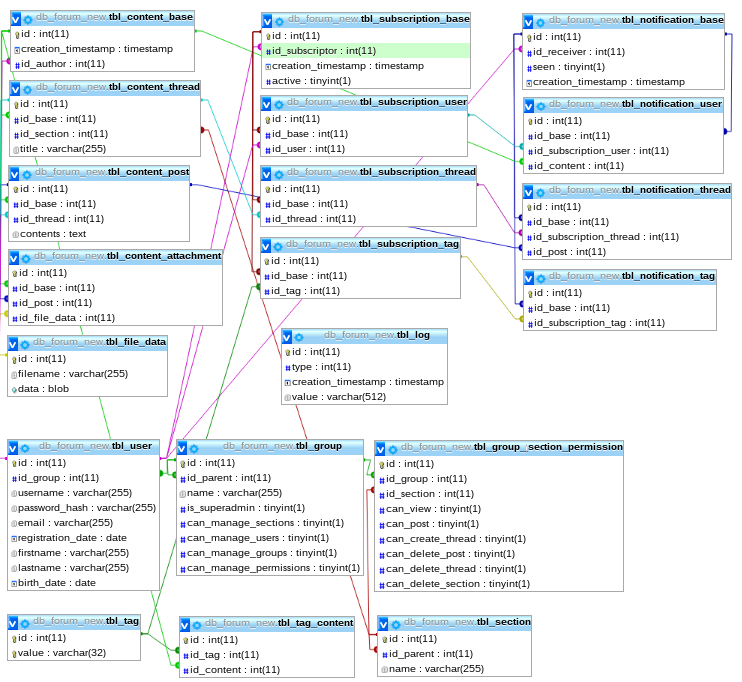
\includegraphics[width=1\textwidth]{logics}
                \end{figure}
                
                \newpage

        \chapter{SQL}

            \section{Database setup}

                veeForum is supposed to be installed on a clean instance of MySQL server. The following script correctly initializes the required database and cleans any previous version of veeForum.

                \printSQLTablepage{00_db.sql}{db}
                    This script is meant to be run once to create and initialize from scratch the whole MySQL veeForum backend.
                    Therefore, we drop the database if exists and re-create it.

                \newpage

            \section{Tables}

                A big amount of tables is required to make veeForum satisfy all requirements. Every table in the project is documented in the following section - the full \emph{DDL} commented code and an explanation is provided for every table.

                \printSQLTablepage{01_tblLog.sql}{log}
                    The \emph{log} table is a simple non-relational list of log messages that can be used for debugging and security purposes.

                \newpage

                \printSQLTablepage{02_tblTag.sql}{tag}
                    The \emph{tag} table is a simple non-relational list of unique tags that can be attached to user-created content.

                \newpage

                \printSQLTablepage{03_tblGroup.sql}{group}
                    The \emph{group} table defines the groups users can belong to. Every row defines a different group and assigns forum-wide permissions to them.
                    Groups can inherit from each other thanks to the \mintinline{sql}{id_parent} field, which is the id of the parent group and can be \mintinline{sql}{NULL}.

                    \begin{figure}[!htb]
                    \caption{Group parenthood relationship.}
                    \centering
                    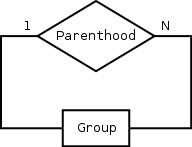
\includegraphics[width=0.5\textwidth]{td/03group}
                    \end{figure}

                \newpage

                \printSQLTablepage{04_tblUser.sql}{user}
                    The \emph{group} table contains the users registered to the forum system. Every user \emph{needs} to belong to a group, whose id is stored in \mintinline{sql}{id_group}.
                    Every row stores user credentials data and personal info.

                    \begin{figure}[!htb]
                    \caption{User-group relationship.}
                    \centering
                    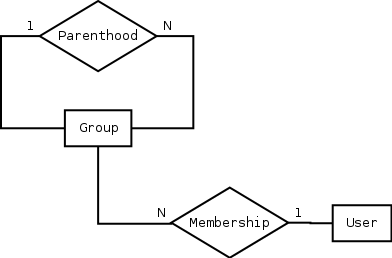
\includegraphics[width=0.5\textwidth]{td/04user}
                    \end{figure}

                \newpage

                \printSQLTablepage{05_tblSection.sql}{section}
                    The \emph{section} table contains all forum sections, defining the base hierarchy for content. Sections have a name and can inherit from each other thanks to the \mintinline{sql}{id_parent} field, which is the id of the parent section and can be \mintinline{sql}{NULL}.

                    \begin{figure}[!htb]
                    \caption{Section parenthood relationship.}
                    \centering
                    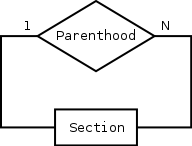
\includegraphics[width=0.5\textwidth]{td/05section}
                    \end{figure}

                \newpage

                \printSQLTablepage{06_tblFileData.sql}{fileData}
                    The \emph{fileData} table stores binary data and a filename for attachments. It makes use of the \mintinline{sql}{blob} MySQL data type to directly store binary data in the database backend.

                \newpage

                \printSQLTablepage{07_tblContentBase.sql}{contentBase}
                    The \emph{contentBase} table defines the base entity of the content inheritance tree. Derived content types are: \emph{threads}, \emph{posts} and \emph{attachments}.
                    All content types share a \mintinline{sql}{creation_timestamp} and an author, identified by \mintinline{sql}{id_author}.

                    \begin{figure}[!htb]
                    \caption{Content specializations.}
                    \centering
                    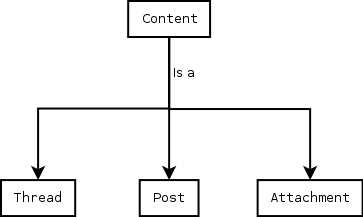
\includegraphics[width=0.5\textwidth]{td/07contentbase}
                    \end{figure}

                \newpage

                \printSQLTablepage{08_tblContentThread.sql}{contentThread}
                    Content specialization for \emph{threads}. A thread belongs to a section (identified by \mintinline{sql}{id_section}) and has a \mintinline{sql}{title}.
                    The base content instance is identified by \mintinline{sql}{id_base}.

                \newpage

                \printSQLTablepage{09_tblContentPost.sql}{contentPost}
                    Content specialization for \emph{posts}. A post belongs to a thread (identified by \mintinline{sql}{id_thread}) and has text \mintinline{sql}{contents}.
                    The base content instance is identified by \mintinline{sql}{id_base}.

                \newpage

                \printSQLTablepage{10_tblContentAttachment.sql}{contentAttachment}
                    Content specialization for \emph{attachments}. An attachment belongs to a post (identified by \mintinline{sql}{id_post}) and points to a specific file data instance \mintinline{sql}{id_file_data}.
                    The base content instance is identified by \mintinline{sql}{id_base}.

                \newpage

                \printSQLTablepage{11_tblSubscriptionBase.sql}{subscriptionBase}
                    The \emph{subscriptionBase} table defines the base entity of the subscription inheritance tree. Derived subscription types are: \emph{thread subscriptions}, \emph{user subscriptions} and \emph{tag subscriptions}.
                    All subscription types share a \mintinline{sql}{creation_timestamp} (beginning of the subscription), a subscriptor (identified by \mintinline{sql}{id_subscriptor}) and an \mintinline{sql}{active} flag that can be turned on and off from the web interface by the subscriptor.

                    \begin{figure}[!htb]
                    \caption{Subscription specializations.}
                    \centering
                    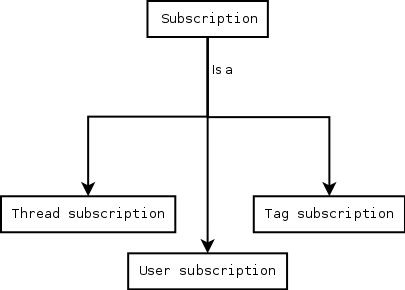
\includegraphics[width=0.5\textwidth]{td/11subscriptionbase}
                    \end{figure}

                \newpage

                \printSQLTablepage{12_tblSubscriptionThread.sql}{subscriptionThread}
                    Subscription specialization for \emph{thread subscriptions}. Allows to track a thread (identified by \mintinline{sql}{id_thread}) for new content additions.
                    The base subscription instance is identified by \mintinline{sql}{id_base}.

                \newpage

                \printSQLTablepage{13_tblSubscriptionUser.sql}{subscriptionUser}
                    Subscription specialization for \emph{user subscriptions}. Allows to track an user (identified by \mintinline{sql}{id_user}) for new content additions.
                    The base subscription instance is identified by \mintinline{sql}{id_base}.

                \newpage

                \printSQLTablepage{14_tblSubscriptionTag.sql}{subscriptionTag}
                    Subscription specialization for \emph{tag subscriptions}. Allows to track a tag (identified by \mintinline{sql}{id_tag}) for new content additions.
                    The base subscription instance is identified by \mintinline{sql}{id_base}.

                \newpage

                \printSQLTablepage{15_tblNotificationBase.sql}{notificationBase}
                    The \emph{notificationBase} table defines the base entity of the notification inheritance tree. Derived notification types are: \emph{thread notifications}, \emph{user notifications} and \emph{tag notifications}.
                    All notifications types share a \mintinline{sql}{seen} flag (which is set to \mintinline{sql}{true} if the receiver seen a particular notification), a receiver (identified by \mintinline{sql}{id_receiver}) and a \mintinline{sql}{creation_timestamp}.

                    Notifications are created from subscriptions, using triggers.

                    \begin{figure}[!htb]
                    \caption{Notification specializations.}
                    \centering
                    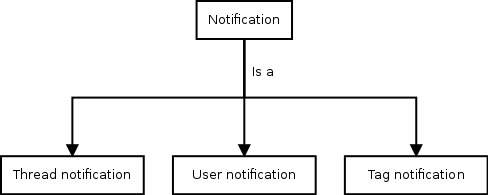
\includegraphics[width=0.5\textwidth]{td/15notificationbase}
                    \end{figure}

                \newpage

                \printSQLTablepage{16_tblNotificationUser.sql}{notificationUser}
                    Notification specialization for \emph{user notifications}. Generated when a tracked user creates new content. Points to the subscription that generated the notification (identified by \mintinline{sql}{id_subscription_user}) and to the created content (identified by \mintinline{sql}{id_content}).
                    The base notification instance is identified by \mintinline{sql}{id_base}.

                \newpage    

                \printSQLTablepage{17_tblNotificationThread.sql}{notificationThread}
                    Notification specialization for \emph{thread notifications}. Generated when new content is added to a tracked thread. Points to the subscription that generated the notification (identified by \mintinline{sql}{id_subscription_thread}) and to the created content (identified by \mintinline{sql}{id_content}).
                    The base notification instance is identified by \mintinline{sql}{id_base}.

                \newpage

                \printSQLTablepage{18_tblNotificationTag.sql}{notificationTag}
                    Notification specialization for \emph{tag notifications}. Generated when new content is labeled with the tracked tag. Points to the subscription that generated the notification (identified by \mintinline{sql}{id_subscription_tag}) and to the created content (identified by \mintinline{sql}{id_content}).
                    The base notification instance is identified by \mintinline{sql}{id_base}.

                \newpage

                \printSQLTablepage{19_tblTagContent.sql}{tagContent}
                    The \emph{tagContent} table labels content to tags.
                    It is a \emph{N to N} relationship table.

                    \begin{figure}[!htb]
                    \caption{Tag-content relationship.}
                    \centering
                    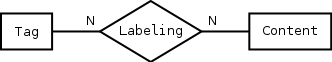
\includegraphics[width=0.5\textwidth]{td/19tagcontent}
                    \end{figure}

                \newpage

                \printSQLTablepage{20_tblGroupSectionPermission.sql}{groupSectionPermission}
                    The \emph{groupSectionPermission} table links groups to sections, giving users belonging to the selected group a set of permissions for the selected section.
                    It is a \emph{N to N} relationship table.

                \newpage

            \section{Stored procedures}

                To ensure \emph{maximum performance} and to \emph{minimize coupling} with the PHP backend, the logic of the forum system is, where possible, implemented with SQL \emph{stored procedures}.
                A stored procedure is a subroutine available to applications that access a relational database system, and it is actually stored in the database data dictionary.

                \printSQLTablepage{21_procsMkContent.sql}{mkContent}
                    The procedures in the code listed above deal with the creation of content. To create content, it is necessary to instantiate both a \mintinline{sql}{content_base} row and a specialization data row.
                    These procedures automatically create both the required rows and make sure they relate to each other correctly, thanks to the \mintinline{sql}{LAST_INSERT_ID()} MySQL function.

                    \begin{itemize}
                        \item \mintinline{sql}{mk_content_base}: creates a content base record and returns its id.
                        \item \mintinline{sql}{mk_content_thread}: calls \mintinline{sql}{mk_content_base}, then creates a thread specialization row linked to it.
                        Takes the author id and title of the thread as input parameters.
                        \item \mintinline{sql}{mk_content_post}: calls \mintinline{sql}{mk_content_base}, then creates a thread specialization row linked to it.
                        Takes the author id and id of the parent thread as input parameters.
                        \item \mintinline{sql}{mk_content_attachment}: calls \mintinline{sql}{mk_content_base}, then creates a thread specialization row linked to it.
                        Takes the author id and id of the parent post as input parameters.
                    \end{itemize}

                \newpage

                \printSQLTablepage{22_procsMkSubscription.sql}{mkSubscription}
                    The procedures in the code listed above deal with the creation of subscriptions. To create subscriptions, it is necessary to instantiate both a \mintinline{sql}{subscription_base} row and a specialization data row.
                    These procedures automatically create both the required rows and make sure they relate to each other correctly, thanks to the \mintinline{sql}{LAST_INSERT_ID()} MySQL function.

                    \begin{itemize}
                        \item \mintinline{sql}{mk_subscription_base}: creates a subscription base record and returns its id.
                         \item \mintinline{sql}{mk_subscription_user}: calls \mintinline{sql}{mk_subscription_base}, then creates a user specialization row linked to it.
                        Takes the subscriptor id and id of the user as input parameters.
                        \item \mintinline{sql}{mk_subscription_thread}: calls \mintinline{sql}{mk_subscription_base}, then creates a thread specialization row linked to it.
                        Takes the subscriptor id and id of the thread as input parameters.
                        \item \mintinline{sql}{mk_subscription_tag}: calls \mintinline{sql}{mk_subscription_base}, then creates a tag specialization row linked to it.
                        Takes the subscriptor id and id of the tag as input parameters.
                    \end{itemize}

                \newpage

                \printSQLTablepage{23_procsMkNotification.sql}{mkNotification}
                     The procedures in the code listed above deal with the creation of notifications. To create notifications, it is necessary to instantiate both a \mintinline{sql}{notification_base} row and a specialization data row.
                    These procedures automatically create both the required rows and make sure they relate to each other correctly, thanks to the \mintinline{sql}{LAST_INSERT_ID()} MySQL function.

                    \begin{itemize}
                        \item \mintinline{sql}{mk_notification_base}: creates a notification base record and returns its id.
                         \item \mintinline{sql}{mk_notification_user}: calls \mintinline{sql}{mk_notification_base}, then creates a user specialization row linked to it.
                        Takes the notification receiver id, the user subscription id and id of the new content as input parameters.
                        \item \mintinline{sql}{mk_notification_thread}: calls \mintinline{sql}{mk_notification_base}, then creates a thread specialization row linked to it.
                        Takes the notification receiver id, the thread subscription id and id of the new content as input parameters.
                        \item \mintinline{sql}{mk_notification_tag}: calls \mintinline{sql}{mk_notification_base}, then creates a tag specialization row linked to it.
                        Takes the notification receiver id, the tag subscription id and id of the new content as input parameters.
                    \end{itemize}

                \newpage

                \printSQLTablepage{24_procsUtils.sql}{utils}
                    The code listed above is composed of several utility stored procedures.

                    \begin{itemize}
                        \item \mintinline{sql}{get_subscriptor}: takes a \emph{subscription base id} as an input parameter and returns the id of the subscriptor.
                        \item \mintinline{sql}{check_notification_unseen_existance_user}: takes a \emph{subscriptor id} and a \emph{target subscribed user id} as input parameters and returns \mintinline{sql}{true} if an unseen user notification with the passed parameters exists.
                        \item \mintinline{sql}{check_notification_unseen_existance_thread}: takes a \emph{subscriptor id} and a \emph{target subscribed thread id} as input parameters and returns \mintinline{sql}{true} if an unseen thread notification with the passed parameters exists.
                        \item \mintinline{sql}{check_notification_unseen_existance_tag}: takes a \emph{subscriptor id} and a \emph{target subscribed tag id} as input parameters and returns \mintinline{sql}{true} if an unseen tag notification with the passed parameters exists.                        
                    \end{itemize}

                \newpage

                \printSQLTablepage{25_procGNUser.sql}{gNUser}
                    The stored procedure listed above deals with the \emph{generation of user notifications}. It is automatically called by the \mintinline{sql}{trg_notifications_user} trigger, which fires after the addition of new content to the system.

                    The procedure takes the \emph{last added content id} and its \emph{author id} as input parameters, and generates (if matching subscriptions exists) notification records for every subscriptor.

                    The code makes use of \emph{complex MySQL features} like \emph{cursors}, \emph{variable declarations} and \emph{loops}.
                    These features are required to efficiently traverse the subscription hierarchies and retrieve the necessary identifiers.

                    To generate the notifications, the \mintinline{sql}{get_subscriptor} and \mintinline{sql}{mk_notification_user} procedures are called inside the loop, for each matching subscriptor.

                \newpage

                \printSQLTablepage{26_procGNThread.sql}{gNThread}
                    The stored procedure listed above deals with the \emph{generation of thread notifications}. It is automatically called by the \mintinline{sql}{trg_notifications_thread} trigger, which fires after the addition of new content to the system.

                    The procedure takes the \emph{last added post id} and its \emph{parent thread id} as input parameters, and generates (if matching subscriptions exists) notification records for every subscriptor.

                    The code makes use of \emph{complex MySQL features} like \emph{cursors}, \emph{variable declarations} and \emph{loops}.
                    These features are required to efficiently traverse the subscription hierarchies and retrieve the necessary identifiers.

                    To generate the notifications, the \mintinline{sql}{get_subscriptor} and \mintinline{sql}{mk_notification_thread} procedures are called inside the loop, for each matching subscriptor.

                \newpage

                \printSQLTablepage{27_procGNTag.sql}{gNTag}
                    The stored procedure listed above deals with the \emph{generation of tag notifications}. It is automatically called by the \mintinline{sql}{trg_notifications_tag} trigger, which fires after the addition of new content to the system.

                    The procedure takes the \emph{last added content's tag id} and its \emph{content base id} as input parameters, and generates (if matching subscriptions exists) notification records for every subscriptor.

                    The code makes use of \emph{complex MySQL features} like \emph{cursors}, \emph{variable declarations} and \emph{loops}.
                    These features are required to efficiently traverse the subscription hierarchies and retrieve the necessary identifiers.

                    To generate the notifications, the \mintinline{sql}{get_subscriptor} and \mintinline{sql}{mk_notification_tag} procedures are called inside the loop, for each matching subscriptor.

                \newpage

                \printSQLTablepage{28_procCalcPrivs.sql}{calcPrivs}
                    The \mintinline{sql}{calculate_final_privileges} stored procedure takes an \emph{user id} input parameter and traverses its \emph{user/group hierarchy} recursively, returning the final system-wide privilege bit set of the user.

                    The bit set contains the following privileges:

                    \begin{itemize}
                        \item \mintinline{sql}{v_is_superadmin}: \mintinline{sql}{true} if the user is a super administrator.
                        \item \mintinline{sql}{v_can_manage_sections}: \mintinline{sql}{true} if the user can manage (add/edit/remove) sections.
                        \item \mintinline{sql}{v_can_manage_users}: \mintinline{sql}{true} if the user can manage (add/edit/remove) users.
                        \item \mintinline{sql}{v_can_manage_groups}: \mintinline{sql}{true} if the user can manage (add/edit/remove) group hierarchies.
                        \item \mintinline{sql}{v_can_manage_permissions}: \mintinline{sql}{true} if the user can manage (add/edit/remove) permission hierarchies.
                    \end{itemize}

                \newpage

                \printSQLTablepage{29_procCalcPerms.sql}{calcPerms}
                    The \mintinline{sql}{calculate_final_permissions} stored procedure takes an \emph{user id} and a \emph{section id} as input parameters and traverses the user's \emph{user/group hierarchy} recursively, calculating and returning the final user permissions related to the passed section.

                    The calculated permission set (a bit set) contains the following boolean values:

                    \begin{itemize}
                        \item \mintinline{sql}{v_can_view}: \mintinline{sql}{true} if the user can view/access the section.
                        \item \mintinline{sql}{v_can_post}: \mintinline{sql}{true} if the user can post in threads existing in the section.
                        \item \mintinline{sql}{v_can_create_thread}: \mintinline{sql}{true} if the user can create threads in the section.
                        \item \mintinline{sql}{v_can_delete_post}: \mintinline{sql}{true} if the user can delete posts inside the section threads.
                        \item \mintinline{sql}{v_can_delete_thread}: \mintinline{sql}{true} if the user can delete threads inside the section.
                        \item \mintinline{sql}{v_can_delete_section}: \mintinline{sql}{true} if the user can delete the section and its subsections.
                    \end{itemize}

                \newpage

            \section{Triggers}

                \printSQLTablepage{90_trgNotifications.sql}{notifications}
                    These triggers deal with \emph{notification generation}.

                    \begin{itemize}
                        \item \mintinline{sql}{trg_notifications_user}: generates a notification when a tracked user creates content.
                        \item \mintinline{sql}{trg_notifications_thread}: generates a notification when a post is added to a tracked thread.
                        \item \mintinline{sql}{trg_notifications_tag}: generates a notification when content with the tracked tag is created.
                    \end{itemize}

                \newpage

                \printSQLTablepage{91_trgDelContentBase.sql}{contentBase}
                    These triggers deal with content deletion and cleanup.

                    The \mintinline{sql}{trg_del_content_base_thread}, \mintinline{sql}{trg_del_content_base_post}, and \mintinline{sql}{trg_del_content_base_attachment} triggers automatically delete the content base instance upon derived content instance deletion.

                    The \mintinline{sql}{trg_del_ntf_user_on_post_del} and \mintinline{sql}{trg_del_ntf_thread_on_post_del} triggers delete notifications pointing to content that is about to get deleted.

                \newpage

                \printSQLTablepage{92_trgDelSubscriptionBase.sql}{subscriptionBase}
                    These triggers deal with subscription base instance automatic deletion upon derived instance deletion.

                \newpage

                \printSQLTablepage{93_trgDelNotificationBase.sql}{notificationBase}
                     These triggers deal with notification base instance automatic deletion upon derived instance deletion.

                \newpage

                \printSQLTablepage{94_trgDelSubscriptionNtf.sql}{subscriptionNtf}
                    These triggers delete all notification belonging to a subscription that's about to be deleted.

                \newpage

                \printSQLTablepage{95_trgDelSubCnt.sql}{delSubCnt}
                    These triggers delete all subscriptions pointing to content that's about to be deleted.

                \newpage

            \section{Database test data inizialization}

                \printSQLTablepage{99_initialize.sql}{initialize}
                    The \mintinline{sql}{initialize} script generates initial data to allow administrator login and forum system testing.

                    The test data consists of two test users and an empty section.

                    One of the users subscribes to the other one, in order to quickly test the notification system.

                \newpage

        \chapter{PHP}

            \emph{Object-oriented design} will be used as much as possible in the PHP5 backend code. The web application will be divided in two major modules: \emph{library} and \emph{core}.

            The library module will contain functions and classes used throughout the whole application.
            
            The web module will contain the actual web pages, divided in individual self-contained modules. 

            \section{Library module}

                The \emph{library PHP module} interfaces with the database, provides HTML-generation function and has additional utilities used in the core web application implementation.

                \emph{Session-stored variables} will be managed through a static \mintinline{php}{Session} class, using statically-stored keys, creating a safe interface and making debugging easier.

                \emph{Debugging} will be handled through a static \mintinline{php}{Debug} class. Logging of errors and query information can be enabled and disabled from administrators, and will be automatically displayed using AJAX.

                The \emph{database connection} will be managed using the \mintinline{php}{mysqli} PHP5 module. Every global database operation such as queries and connection will be wrapped in a safe interface that allows easy debugging and prevents security breaches.

                \emph{Privileges and permissions} will be loaded/saved from/to the database using bitset-like class instances that support all basic bitset operations. Their underlying implementation is separated from their API – this allows developers to optimize or modify the bit storage without affecting code in the web module.

                AJAX and shortcut functions for HTML generation will be handled through the \mintinline{php}{Gen} static class and the \mintinline{php}{Actions} static class.

                AJAX requests will directly call functions (if valid) from the Actions class, which return HTML, JSON, or plain text. Gen functions will be used from the web module to make the page structure more modular and avoid markup duplication.

                Signing in and out and current user data will be managed from the \mintinline{php}{Credentials} static class. It will contain easy-to-use functions to check privileges and permissions, and also to handle login/logout.

                Last, but not least, \emph{database table interaction} will be handled by a very developer-friendly object-oriented interface. Every table in the database will have a corresponding class, derived from a generic Table class.

                The \mintinline{php}{Table} class provides an object-oriented interface for common queries and \emph{CRUD operations}. It also provides some very convenient methods to perform an action on every row matching a specific predicate or every row that’s part of a hierarchy.

                Their usage, combined with \emph{PHP5 lambda functions}, will make usually complex hierarchy-traversing operations easy to write and debug. These functions are available for every table in the database. The classes derived from \mintinline{php}{Table} will implement functionality that is unique for specific database entities. Insertion and edit fields will be specified in the constructor of these classes, allowing the developer to use a very convenient and clean syntax for the insertion/editing of table rows.

                \subsection{settings}

                    The \emph{settings} submodule uses an intermediate server JSON storage to load and save system-wide settings.

                    The JSON file contains two properties:

                    \begin{itemize}
                        \item \mintinline{php}{forumName}: name of the forum, displayed in the navigation bar and HTML \mintinline{html}{<head>} tag.
                        \item \mintinline{php}{defaultGroup}: id of the group newly registered users are inserted into.
                    \end{itemize}

                    The properties mentioned above are accessible through the following PHP interface:

                    \begin{minted}[mathescape, linenos, numbersep=5pt, gobble=2, frame=lines, framesep=2mm, fontsize=\footnotesize]{php}
    <?php

    class Settings
    {
        // Initialize settings
        public static function init();

        // Load/save settings from/to JSON
        public static function loadFromFile();
        public static function saveToFile();

        // Get/set settings
        public static function setForumName($mX);
        public static function setDefaultGroup($mX);
        public static function getForumName();
        public static function getDefaultGroup();
    }

    ?>
                    \end{minted}

                \subsection{session}

                    The \emph{session} submodule provides useful functions to manage session-stored variables in a convenient and type-safe way.

                    An enumeration-like class is defined for session key-value pairs keys:

                    \begin{minted}[mathescape, linenos, numbersep=5pt, gobble=2, frame=lines, framesep=2mm, fontsize=\footnotesize]{php}
    <?php

    class SK
    {
        // Example keys
        public static $userID = "A1";
        public static $debugLog = "A2";
        public static $debugEnabled = "A3";
        public static $pageID = "pageid";
        public static $threadID = "threadid";
    }

    ?>
                    \end{minted}

                    Accessing session variables is then done through the following PHP static interface:


                    \begin{minted}[mathescape, linenos, numbersep=5pt, gobble=2, frame=lines, framesep=2mm, fontsize=\footnotesize]{php}
    <?php

    class Session
    {
        // Initialize session
        public static function init();

        // Get/set session variables
        public static function get($mX);
        public static function set($mX, $mVal);
    }

    ?>
                    \end{minted}

                \subsection{debug}

                    The \emph{debug} submodule gives the developer a convenient interface to toggle debugging features and access the debug log.

                    \begin{minted}[mathescape, linenos, numbersep=5pt, gobble=2, frame=lines, framesep=2mm, fontsize=\footnotesize]{php}
    <?php

    class Debug
    {
        // Toggle debug mode
        public static function setEnabled($mX);
        public static function isEnabled();

        // Clear log
        public static function clear();

        // Logging functions
        public static function lo($mX);
        public static function loLn();
        public static function echoLo();
    }

    ?>
                        \end{minted}


                \subsection{db}

                     The \emph{db} submodule provides a friendly interface to the database backend, abstracting most common queries and correctly handling quoted or null arguments.
                     Its public interface is shown below:

                    \begin{minted}[mathescape, linenos, numbersep=5pt, gobble=2, frame=lines, framesep=2mm, fontsize=\footnotesize]{php}
    <?php

    class DB
    {
        // Connects to the database
        public static function connect();

        // Executes a query and returns its result
        public static function query($mX);

        // Returns the last inserted ID in the database
        public static function getInsertedID();

        // Returns a correctly escaped version of a string
        public static function esc($mX);

        // Returns a correctly quoted version of a value
        public static function v($mX);
    }

    ?>
                    \end{minted}


                \subsection{privs}

                    The \emph{privs} submodule deals with system-wide privileges. Privileges are handled as bitsets.

                    The \mintinline{php}{Privs} static enumeration-like class assigns an unique integer to every privilege bit:

                    \begin{minted}[mathescape, linenos, numbersep=5pt, gobble=2, frame=lines, framesep=2mm, fontsize=\footnotesize]{php}
    <?php

    class Privs
    {
        const count = 5;

        const isSuperAdmin = 0;
        const canManageSections = 1;
        const canManageUsers = 2;
        const canManageGroups = 3;
        const canManagePermissions = 4;
    }

    ?>
                    \end{minted}

                    Privilege bitsets are \mintinline{php}{PrivSet} instances. They provide functions available in most bitset implementations.

                    The public interface is shown below:
 
                    \begin{minted}[mathescape, linenos, numbersep=5pt, gobble=2, frame=lines, framesep=2mm, fontsize=\footnotesize]{php}
    <?php

    class PrivSet
    {
        // Variadic constructor - constructs an
        // instance of `PrivSet` with the passed privileges
        public function __construct(...$mPrivs);

        // Instantiates a `PrivSet` from a string
        public static function fromStr($mX);

        // Instantiates a `PrivSet` from a group
        public static function fromGroup($mX);

        // Returns a string representing the current `PrivSet`
        public function toStr();

        // Add/delete a privilege
        public function add($mX);
        public function del($mX);

        // Check availability of a privilege
        public function has($mX);

        // Returns true if this `PrivSet` is equal to another one
        public function isEqualTo($mX);

        // Returns the logical or between two `PrivSet` instances
        public function getOrWith($mX);

        // Returns the logical and between two `PrivSet` instances
        public function getAndWith($mX);
    }

    ?>                        
                    \end{minted}

                \subsection{pages}

                    The \emph{pages} submodule provides a simple framework for web application paging.

                    The \mintinline{php}{PK} static enumeration-like class assigns an unique integer to every page:

                    \begin{minted}[mathescape, linenos, numbersep=5pt, gobble=2, frame=lines, framesep=2mm, fontsize=\footnotesize]{php}
    <?php

    class PK
    {
        public static $sections = 0;
        public static $administration = 1;
        public static $threadView = 2;
    }

    ?>
                    \end{minted}

                    Every page has its own \mintinline{php}{PageData} instance, which stores its URL and required access privileges.

                    \begin{minted}[mathescape, linenos, numbersep=5pt, gobble=2, frame=lines, framesep=2mm, fontsize=\footnotesize]{php}
    <?php

    class PageData
    {
        // Variadic constructor - takes the URL of the page
        // and any number of required privileges as parameters
        public function __construct($mURL, ...$mPrivs);

        // Returns the URL of the apge
        public function getURL();

        // Returns the required access privileges of the page
        public function getPrivs();

        // Returns true if the passed privileges are enough
        // to access the page
        public function canViewWithPrivs($mX);
    }

    ?>
                    \end{minted}

                    All \mintinline{php}{PageData} instances are stored in a static \mintinline{php}{Pages} class:

                    \begin{minted}[mathescape, linenos, numbersep=5pt, gobble=2, frame=lines, framesep=2mm, fontsize=\footnotesize]{php}
    <?php

    class Pages
    {
        // Adds a page to the storage
        // Forwards the variadic arguments to the `PageData` constructor
        public static function add(...$mArgs);

        // Gets a `PageData` by unique page id
        public static function get($mX);

        // Gets or sets the current page in session
        public static function setCurrent($mX);
        public static function getCurrent();
    }

    ?>
                    \end{minted}

                    Web application pages can then be added using the following syntax:

                    \begin{minted}[mathescape, linenos, numbersep=5pt, gobble=2, frame=lines, framesep=2mm, fontsize=\footnotesize]{php}
    <?php

    Pages::add("php/core/content/sections.php");
    Pages::add("php/core/content/adminPanel.php", Privs::isSuperAdmin);
    Pages::add("php/core/content/threadView.php");

    ?>
                    \end{minted}

                \subsection{utils}

                    Self-documenting static class containing various utility functions.

                    \begin{minted}[mathescape, linenos, numbersep=5pt, gobble=2, frame=lines, framesep=2mm, fontsize=\footnotesize]{php}
    <?php

    class Utils
    {
        // Converts an array to a comma-separated-list
        public static function getCSL($mArray);

        // Calculates the hash for a password
        public static function getPwdHash($mX);

        // Returns false if the string is not valid, empty, or
        // only whitespace
        public static function checkEmptyStr($mX, &$mMsg);

        // Returns the parent of the last inserted record in
        // the database (can be null)
        public static function getInsertParent(&$mTbl, $mIDParent);
    }

    ?>
                    \end{minted}                

                \subsection{gen}

                    The \emph{gen} submodule provides a complex HTML generation system that builds a hierarchy of polymorphic PHP class instances.

                    AJAX-enabled HTML can then be generated by traversing the hierarchy recursively.

                    \mintinline{php}{ControlBase} is a class that represents a control hierarchy. Its functions can be used to access/edit the control hierarchy, to move around in the tree or to generate HTML.

                    Shortcut functions starting in \mintinline{php}{in} go one level deeper in the hierarchy.
                    Shortcut functions starting in \mintinline{php}{out} go one level above in the hierarchy.
                    Shortcut functions starting in \mintinline{php}{for} execute a callable object while traversing the hierarchy.

                    \begin{minted}[mathescape, linenos, numbersep=5pt, gobble=2, frame=lines, framesep=2mm, fontsize=\footnotesize]{php}
    <?php

    class ControlBase
    {
        // Add a child to this control
        public function &add(&$mChild);

        // Go one level above
        public function &out();

        // Go to the root of the hierarchy
        public function &root();

        // Parses and includes a PHP file as a child control
        public function &file($mX);

        // Prints the entire hierarchy as HTML
        public function printRoot();

        // Executes the function/lambda for every children
        public function forChildren($mFn);

        // Executes the function/lambda for every children (recursively)
        public function forChildrenRecursive($mFn);

        // Executes the function/lambda for every parent (recursively)
        public function forParentRecursive($mFn);

        // Shortcuts for common HTML elements
        public function &literal(...$mArgs);
        public function &inDiv(...$mArgs);
        public function &inSpan(...$mArgs);
        public function &strong($mX);
        public function &h($mHLevel, $mX);
        public function &hr();
        public function &br();
        public function &inFooter(...$mArgs);
        public function &inA(...$mArgs);
        public function &label($mFor, $mCaption);

        // Shortcuts for common Bootstrap elements
        public function &bsIcon($mIcon);
        public function &inBSLinkBtn($mID, $mClass = '');
        public function &inBSLinkBtnActive($mID, $mOnClick, $mClass = '');
        public function &inBSLinkBtnCloseModal();
        public function &bsLinkBtnAddDismissModal();
        public function &inBSModal($mID);
        public function &inBSModalHeader($mTitle);
        public function &inBSModalBody();
        public function &inBSModalFooter();
        public function &inBSBtnGroup($mClass);
        public function &inBSPanelNoHeader($mClass = '');
        public function &inBSPanelWithHeader($mHeader);
        public function &inBSTable($mID);
        public function &inBSNavbarTextbox($mID, $mCaption);
        public function &bsNavbarTextbox($mID, $mCaption);
        public function &inBSFormTextbox($mID, $mCaption);
        public function &bsFormTextbox($mID, $mCaption);
        public function &bsFormTextarea($mID, $mCaption, $mRows);
    }

    ?>
                    \end{minted}            

                    Complex elements that require additional stored data or special functions can be defined as classes that derive from \mintinline{php}{ControlBase}.

                    \begin{minted}[mathescape, linenos, numbersep=5pt, gobble=2, frame=lines, framesep=2mm, fontsize=\footnotesize]{php}
    <?php

    // Example derived controls
    class Container extends ControlBase;
    class Literal extends ControlBase;
    class HTMLControl extends ControlBase;
    class BSModal extends Container;

    ?>
                    \end{minted}               

                    Here's an example usage of the HTML generation module:

                    \begin{minted}[mathescape, linenos, numbersep=5pt, gobble=2, frame=lines, framesep=2mm, fontsize=\footnotesize]{php}
    <?php 

    (new Container())
        ->h(1, 'Administration')
        ->hr()
        ->inDiv(['class' => 'row'])
            ->file("$rootAP/panelDebug.php")
            ->file("$rootAP/panelGroups.php")
            ->out()
        ->hr()
        ->inDiv(['class' => 'row'])
            ->file("$rootAP/panelGSPerms.php")
            ->file("$rootAP/panelSections.php")
            ->out()
        ->hr()
        ->inDiv(['class' => 'row'])
            ->file("$rootAP/panelUsers.php")
    ->printRoot();

    ?>
                    \end{minted}           

                \subsection{tbl}

                    The \emph{tbl} submodule provides a complex and fully-featured database table wrapping and management system for the PHP backend.

                    Every database table is defined in the PHP backend as a class deriving from \mintinline{php}{Tbl}. 

                    \mintinline{php}{Tbl} is an extremely powerful abstraction that offers developers an huge amount of convenient functions to manage the records of a database table:

                    \begin{minted}[mathescape, linenos, numbersep=5pt, gobble=2, frame=lines, framesep=2mm, fontsize=\footnotesize]{php}
    <?php

    class Tbl
    {
        // Constructs a `Tbl` instance with a specific name
        // and a set of fields for value insertion
        public function __construct($mTblName, ...$mInsertFields);

        // Set the fields required to insert a new value
        public function setInsertFields(...$mFields);

        // Inserts a new record with the passed variadic values in
        // the database
        public function insert(...$mValues);

        // Inserts a new record with the passed variadic values in
        // the database (correctly escapes the passed arguments)
        public function insertValues(...$mValues);

        // Finds a record by ID and updates it
        public function updateByID($mID, $mArray);

        // Returns all records in an array
        public function getAll();

        // Returns all records matching a specific predicate in an array
        public function getWhere($mX);

        // Returns the first record
        public function getFirst($mX);

        // Returns the first record matching a specific predicate
        public function getFirstWhere($mX);

        // Deletes all records matching a specific predicate
        public function deleteWhere($mX);

        // Finds a record by ID and deletes it
        public function deleteByID($mID);

        // Finds a record by ID and deletes its hierarchy, if existing
        public function deleteRecursiveByID($mID);
        
        // Finds and returns a record by ID
        public function findByID($mID);

        // Finds all children of a specific record by ID
        public function findAllByIDParent($mIDParent);

        // Returns true if any record matches the predicate
        public function hasAnyWhere($mX);

        // Returns true if a record with the passed ID exists
        public function hasID($mID);

        // Executes the passed function/lambda on every record
        public function forRows($mFn);

        // Executes the passed function/lambda on every record matching
        // a specific predicate
        public function forWhere($mFn, $mWhere);

        // Executes the passed function/lambda on every child of a
        // record
        public function forChildren($mFn, $mIDParent = null, $mDepth = 0);

        // Executes the passed function/lambda on every parent of a
        // record
        public function forParent($mFn, $mID, $mDepth = 0);
    }

    ?>
                    \end{minted}                

                    Database tables can then be wrapped and instantiated in the following way:

                    \begin{minted}[mathescape, linenos, numbersep=5pt, gobble=2, frame=lines, framesep=2mm, fontsize=\footnotesize]{php}
    <?php

    // ...

    TBS::$log = new TblLog('tbl_log',
        'type', 'creation_timestamp', 'value');

    TBS::$tag = new TblTag('tbl_tag',
        'value');

    TBS::$section = new TblSection('tbl_section',
        'id_parent', 'name');

    TBS::$cntBase = new Tbl('tbl_content_base');
    TBS::$cntThread = new TblCntThread('tbl_content_thread');
    TBS::$cntPost = new TblCntPost('tbl_content_post');
    TBS::$cntAttachment = new TblCntAttachment('tbl_content_attachment');

    // ...

    ?>
                    \end{minted}              
                
                \subsection{sprocs}

                    The \emph{sprocs} submodule provides a powerful and convenient abstraction to manage and call MySQL stored procedures from the PHP backend.

                    Every database stored procedure can be wrapped in a \mintinline{php}{SProc} instance.

                    The user-friendly yet extremely useful \mintinline{php}{SProc} public interface is shown below:

                    \begin{minted}[mathescape, linenos, numbersep=5pt, gobble=2, frame=lines, framesep=2mm, fontsize=\footnotesize]{php}
    <?php

    class SProc
    {
        // Constructs a stored procedure with a specific name,
        // and a number of in/out parameters
        public function __construct($mProcedureName, 
            $mInParamCount, $mOutParamCount);

        // Forwards the variadic arguments to the stored procedure
        // and calls it
        public function call(...$mArgs);

        // Forwards the variadic arguments to the stored procedure
        // and calls it, returning its out parameters in an array
        public function callOut(&$mOutArray, ...$mArgs);
    }

    ?>
                    \end{minted}      

                    Stored procedures can then be instantiated and wrapped in the web application code like this:

                    \begin{minted}[mathescape, linenos, numbersep=5pt, gobble=2, frame=lines, framesep=2mm, fontsize=\footnotesize]{php}          
    <?php

    // ...

    SPRCS::$mkContentThread = new SProc('mk_content_thread', 3, 0);
    SPRCS::$mkContentPost = new SProc('mk_content_post', 3, 0);
    SPRCS::$mkContentAttachment = new SProc('mk_content_attachment', 3, 0);

    SPRCS::$mkSubscriptionUser = new SProc('mk_subscription_user', 2, 0);
    SPRCS::$mkSubscriptionThread = new SProc('mk_subscription_thread', 2, 0);
    SPRCS::$mkSubscriptionTag = new SProc('mk_subscription_tag', 2, 0);

    // ...

    ?>
                    \end{minted}      

            \section{Core module}

                The \emph{core PHP module} contains the implementation of the default \emph{veeForum web application}, which makes use of all the library module features described above.

                Its folder structure is as follows:

                \begin{minted}[mathescape, linenos, numbersep=5pt, gobble=2, frame=lines, framesep=2mm, fontsize=\footnotesize]{bash}
    .
    ├── body
    │   ├── footer.php
    │   ├── loginControls.php
    │   ├── modalInfo.php
    │   ├── modalNotifications.php
    │   ├── navbarContents.php
    │   ├── navbar.php
    │   └── profileControls.php
    ├── body.php
    ├── content
    │   ├── actions.php
    │   ├── adminPanel
    │   │   ├── modalGSPerms.php
    │   │   ├── modalUserActions.php
    │   │   ├── modalUserEdit.php
    │   │   ├── panelDebug.php
    │   │   ├── panelGroups.php
    │   │   ├── panelGSPerms.php
    │   │   ├── panelSections.php
    │   │   ├── panelTags.php
    │   │   └── panelUsers.php
    │   ├── adminPanel.php
    │   ├── forbidden.php
    │   ├── register
    │   │   └── modalRegister.php
    │   ├── sections
    │   │   ├── modalNewPost.php
    │   │   └── modalNewThread.php
    │   ├── sections.php
    │   └── threadView.php
    └── head.php
                \end{minted}

                The \mintinline{php}{body} folder contains the implementation of the main page's modules, such as information/error modals, the navigation bar, etc.

                The \mintinline{php}{content} folder contains several subfolders:

                \begin{itemize}
                    \item \mintinline{php}{adminPanel}: implementation of the administration section and all its modules.
                    \item \mintinline{php}{register}: implementation of the registration interface.
                    \item \mintinline{php}{sections}: implementation of the \emph{new post} and \emph{new thread} interfaces.
                \end{itemize}

                Screenshots of the web interface will be shown in the following chapter, showing the end-result of the combination of the PHP modules.

        \chapter{Web interface}
            
            \begin{figure}[!htb]
            \caption{Main page - user not logged in.}
            \centering
            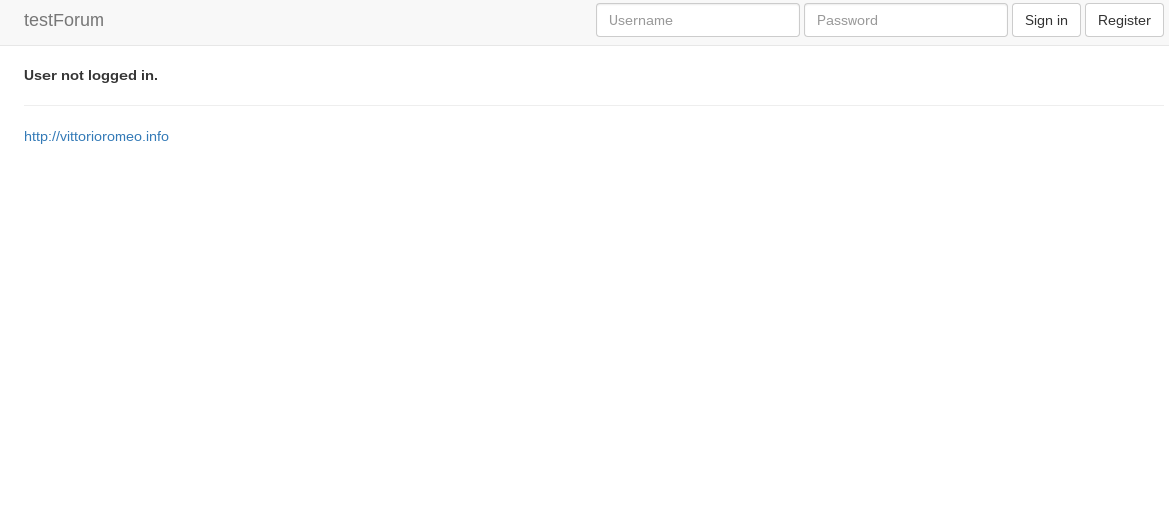
\includegraphics[width=1\textwidth]{u/0}
            \end{figure}

            \begin{figure}[!htb]
            \caption{Registration modal.}
            \centering
            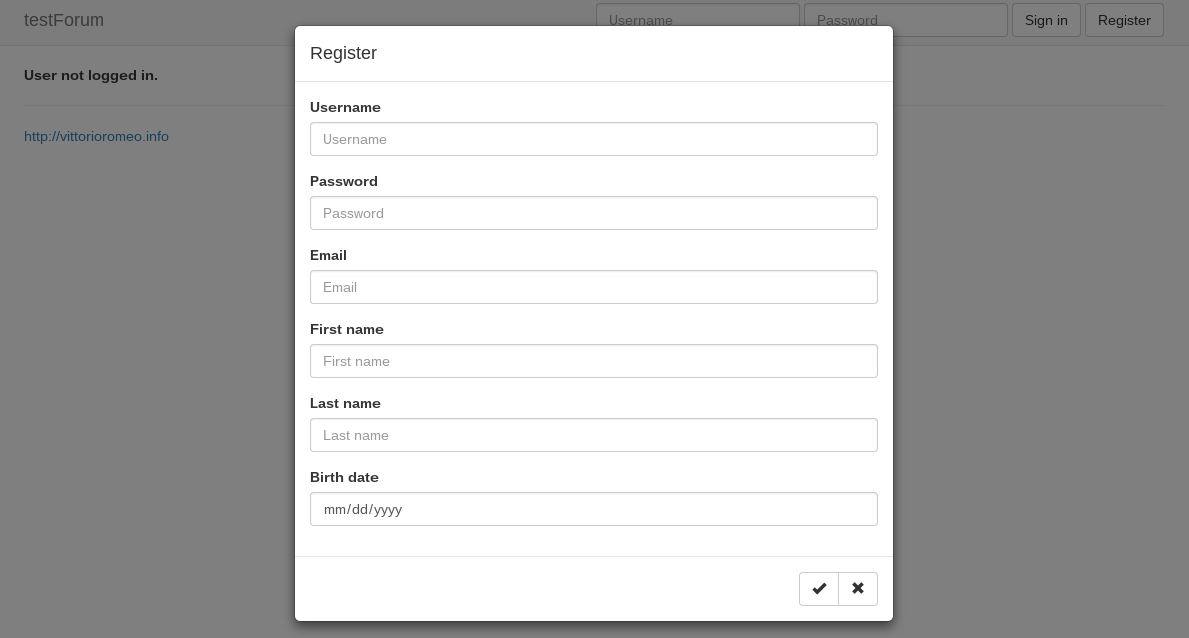
\includegraphics[width=1\textwidth]{u/1}
            \end{figure}

            \begin{figure}[!htb]
            \caption{Main page - user logged in.}
            \centering
            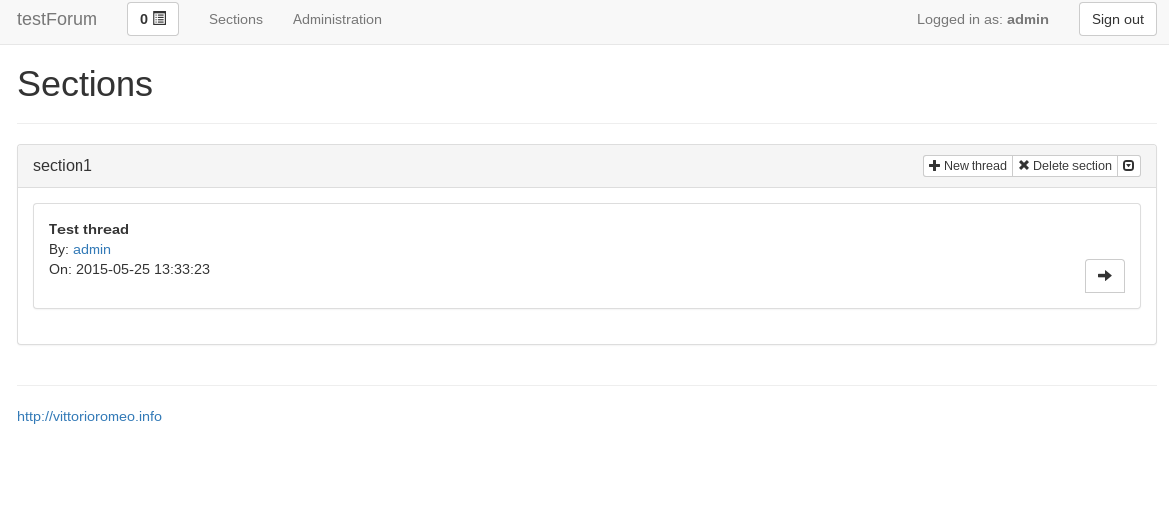
\includegraphics[width=1\textwidth]{u/2}
            \end{figure}

            \begin{figure}[!htb]
            \caption{New thread modal.}
            \centering
            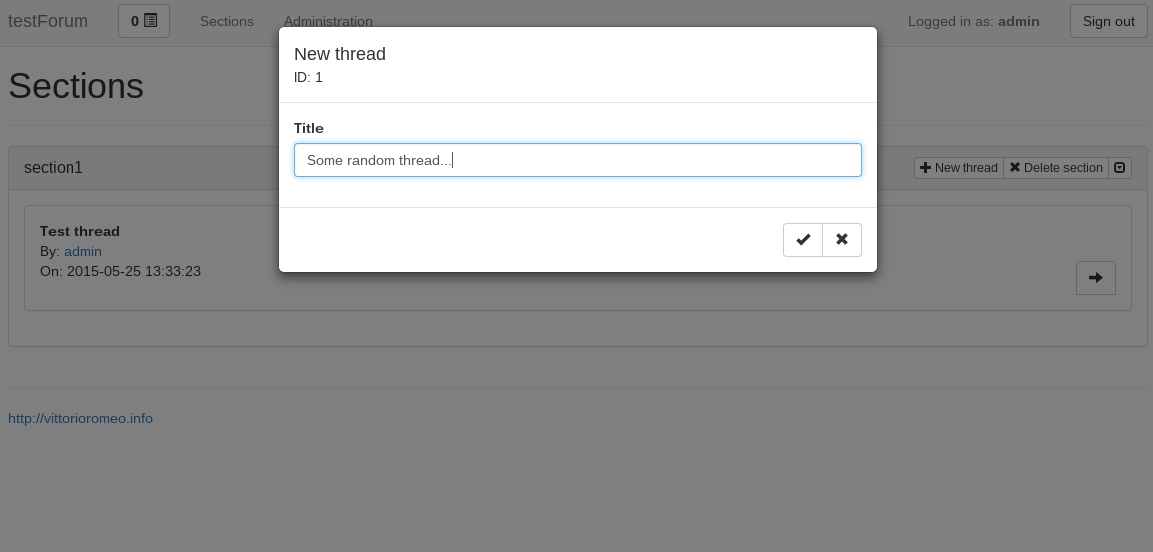
\includegraphics[width=1\textwidth]{u/3}
            \end{figure}

            \begin{figure}[!htb]
            \caption{Thread view page.}
            \centering
            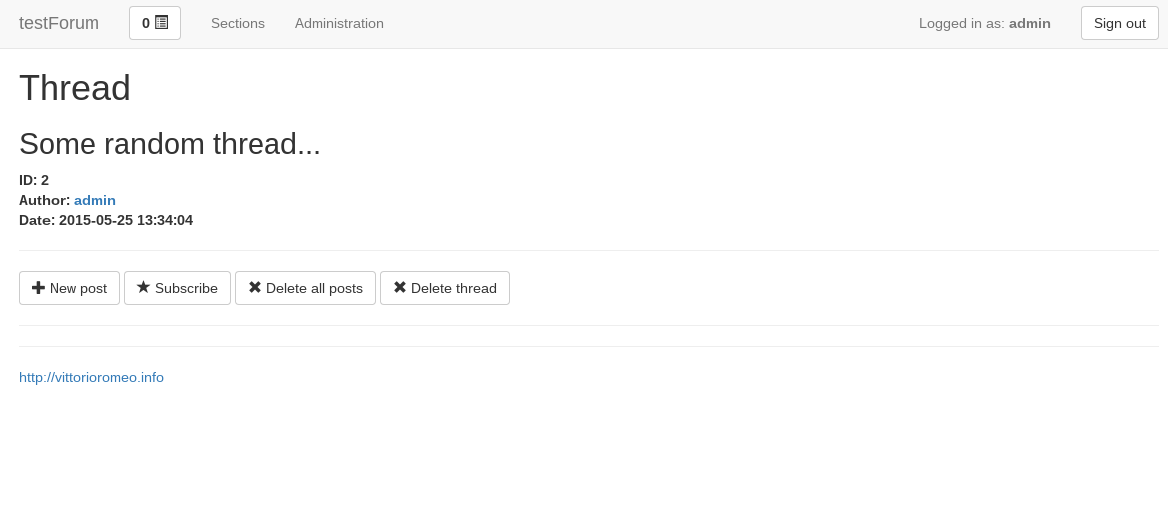
\includegraphics[width=1\textwidth]{u/4}
            \end{figure}

            \begin{figure}[!htb]
            \caption{New post modal.}
            \centering
            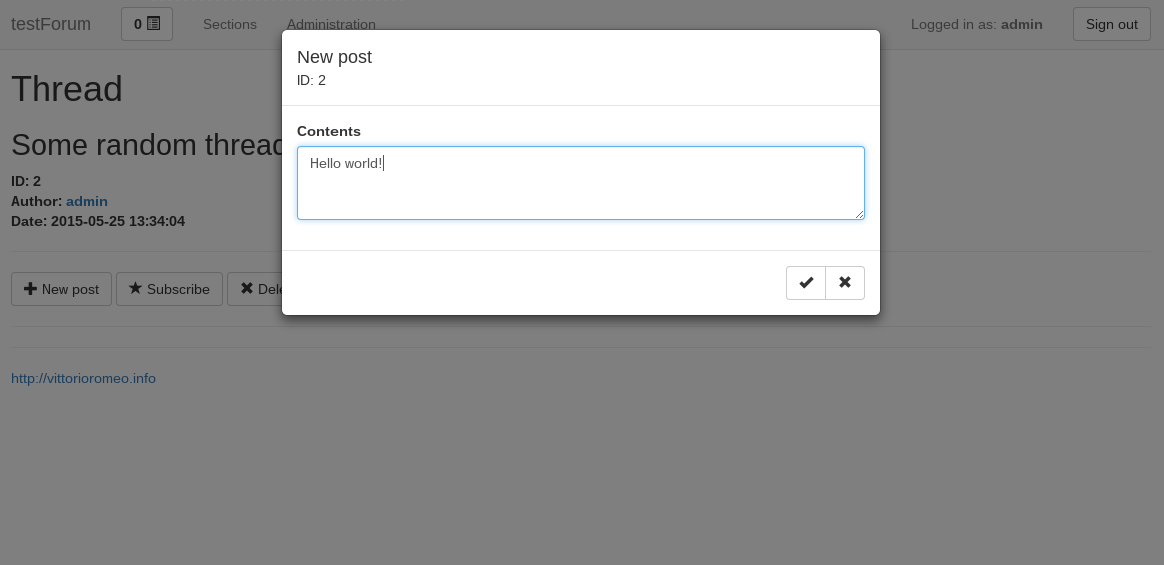
\includegraphics[width=1\textwidth]{u/5}
            \end{figure}

            \begin{figure}[!htb]
            \caption{Thread view page - subscription.}
            \centering
            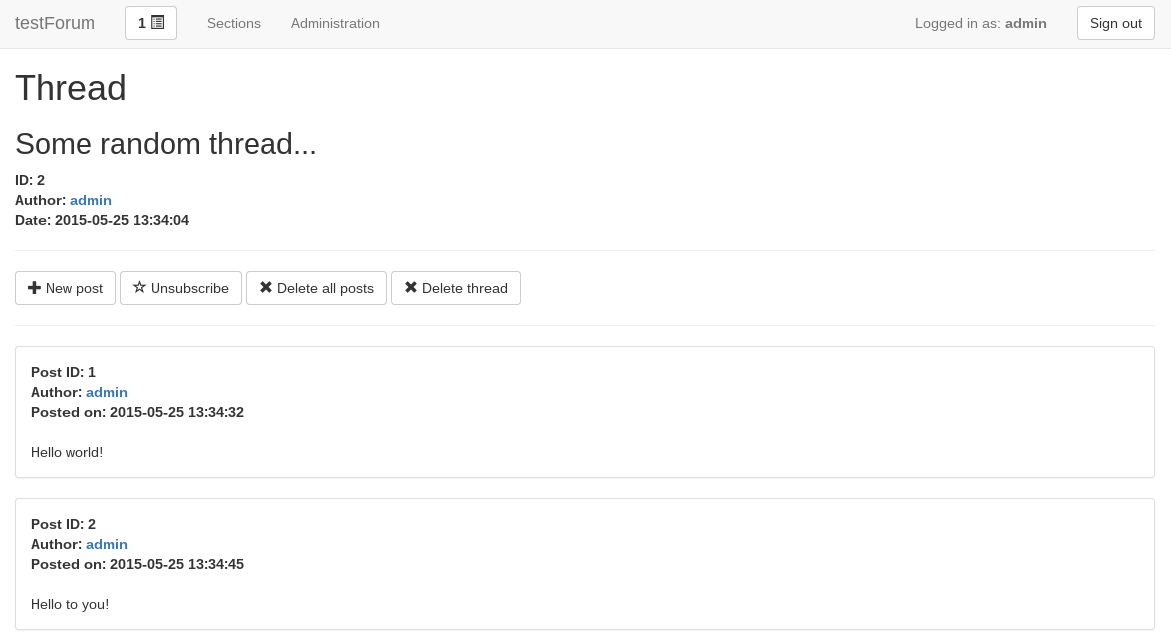
\includegraphics[width=1\textwidth]{u/6}
            \end{figure}

            \begin{figure}[!htb]
            \caption{Notifications modal.}
            \centering
            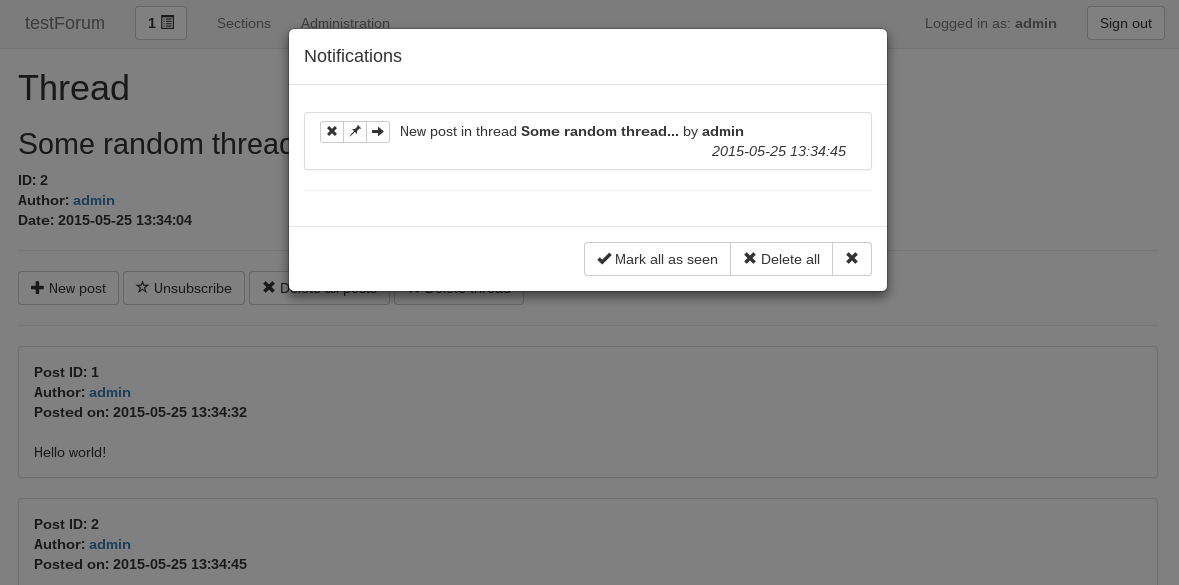
\includegraphics[width=1\textwidth]{u/7}
            \end{figure}

            \begin{figure}[!htb]
            \caption{Administration panel - 1.}
            \centering
            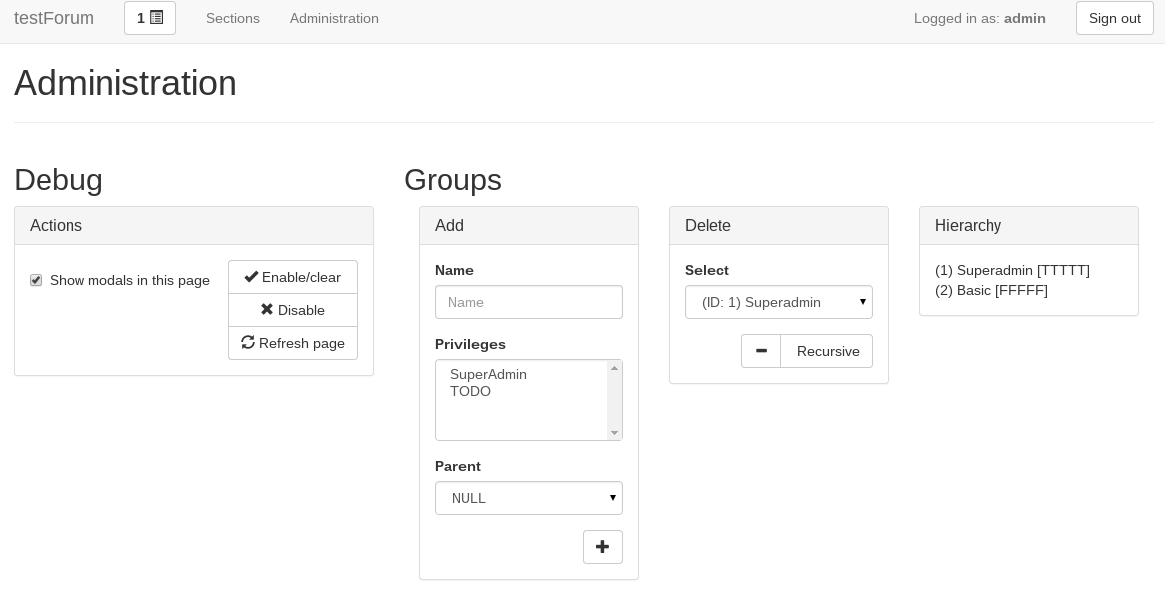
\includegraphics[width=1\textwidth]{u/8}
            \end{figure}

            \begin{figure}[!htb]
            \caption{Administration panel - 2.}
            \centering
            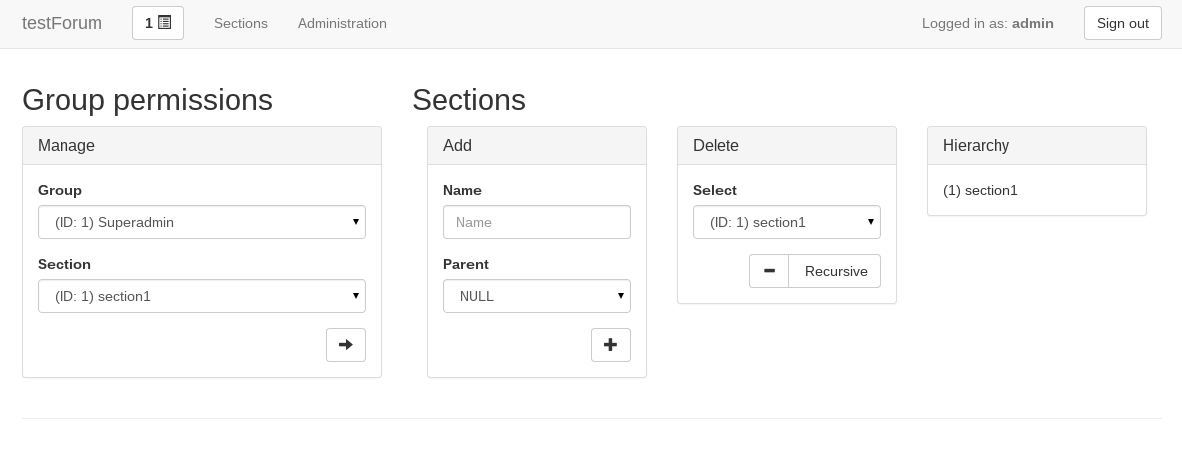
\includegraphics[width=1\textwidth]{u/9}
            \end{figure}

            \begin{figure}[!htb]
            \caption{Administration panel - 3.}
            \centering
            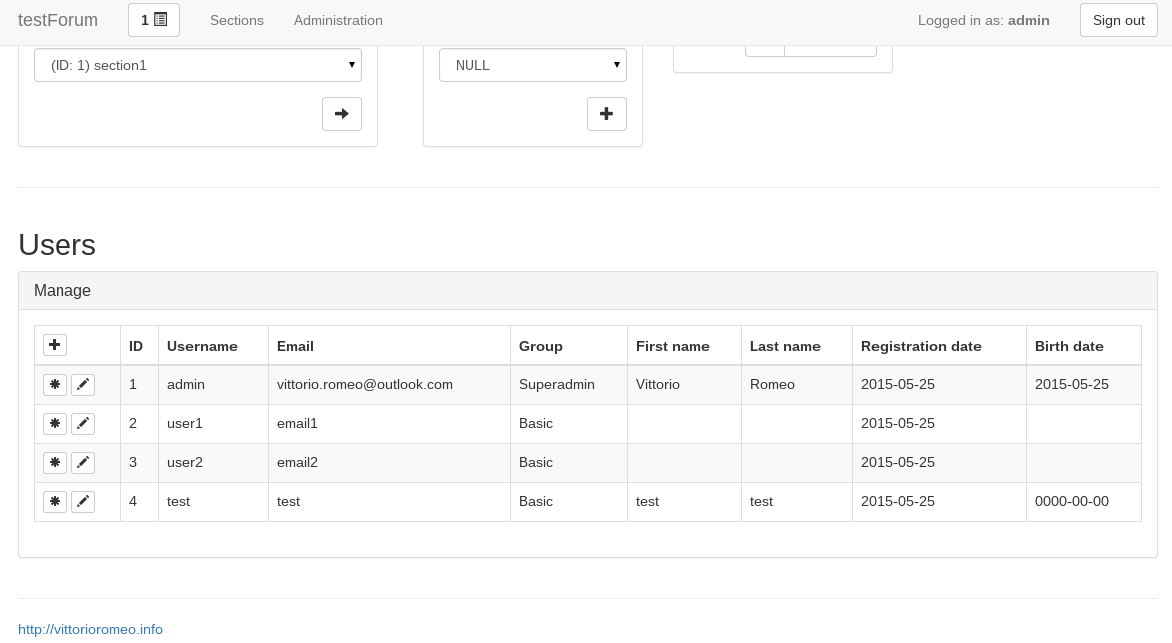
\includegraphics[width=1\textwidth]{u/10}
            \end{figure}


    \part{Conclusion}
        aaa

        \chapter{Final product}
            aaa

        \chapter{What I learned}
            aaa

        \chapter{Future}
            aaa

        \chapter{References}
            aaa

\end{document}
